\documentclass[memoir, 12pt]{report}

\usepackage[top = 2cm, bottom = 1.5cm, left = 2cm, right = 2cm]{geometry}
\usepackage{enumitem}
%\\usepackage{mathtools}
% \usepackage[linesnumbered,ruled,french]{algorithm2e}

%\usepackage[linesnumbered, french]{algorithm2e}
%\usepackage{algorithm2e}

%\usepackage{multibib}
%\newcites{biblio}{Bibliographie}
%\newcites{other}{Autres r\'ef\'erences}
\usepackage{amssymb}
\usepackage{amsmath}
\usepackage{graphicx}
\usepackage{amsfonts}
\usepackage{lmodern}
\usepackage{caption}
\usepackage{subcaption}
\usepackage[babel=true]{csquotes}
\setlength{\fboxrule}{0.01cm}
\setlength{\fboxsep}{0.5cm}
\usepackage{tikz}
\usepackage{lipsum}
\usepackage{setspace}
\usepackage{ragged2e}
\usepackage{url}
\usepackage{float}
%\usepackage[thinlines]{easytable}
\usepackage{hyperref}
\usepackage[export]{adjustbox}
\usepackage{tabularx}
\newcolumntype{b}{X}
\newcolumntype{s}{>{\hsize=.5\hsize}X}
\usepackage{multicol}
%\\usepackage{tabto}
\usepackage{multirow}
\usepackage{colortbl}

% Keywords command
\providecommand{\keywords}[2]
{
  \vspace{1.2cm}
  \textbf{{#1 :}} #2
}

\graphicspath{{figures/}}

%\usepackage{algpseudocode}
%\usepackage[french]{algorithmic}
%\usepackage{algorithmic}
%\usepackage[algcompatible]{algpseudocode}
%\algrenewcommand\alglinenumber[1]{\footnotesize #1}
%\usepackage[table,xcdraw]{xcolor}
\usepackage[normalem]{ulem}
\useunder{\uline}{\ul}{}
\usepackage[french]{babel}
\frenchbsetup{StandardLists=true}

\usepackage{amssymb} 
\usepackage{dsfont}

\usepackage{algorithm}
\usepackage[french]{algorithmic}
\renewcommand{\listalgorithmname}{Liste des algorithmes}
\floatname{algorithm}{Algorithme}
\renewcommand{\algorithmicreturn}{\textbf{retourner}}
\renewcommand{\algorithmicprocedure}{\textbf{procédure}}
\renewcommand{\Not}{\textbf{non}\ }
\renewcommand{\And}{\textbf{et}\ }
\renewcommand{\Or}{\textbf{ou}\ }
\renewcommand{\algorithmicrequire}{\textbf{Entrée:}}
\renewcommand{\algorithmicensure}{\textbf{Sortie:}}
%\renewcommand{\algorithmiccomment}[1]{\{#1\}}
\renewcommand{\algorithmicend}{\textbf{fin}}
\renewcommand{\algorithmicif}{\textbf{si}}
\renewcommand{\algorithmicthen}{\textbf{alors}}
\renewcommand{\algorithmicrepeat}{\textbf{repéter}}
\renewcommand{\algorithmicuntil}{\textbf{tantque}}
\renewcommand{\algorithmicelse}{\textbf{sinon}}
\renewcommand{\algorithmicfor}{\textbf{pour}}
\renewcommand{\algorithmicforall}{\textbf{pour tout}}
\renewcommand{\algorithmicdo}{\textbf{faire}}
\renewcommand{\algorithmicwhile}{\textbf{tant que}}
\newcommand{\algorithmicelsif}{\algorithmicelse\ \algorithmicif}
\newcommand{\algorithmicendif}{\algorithmicend\ \algorithmicif}
\newcommand{\algorithmicendfor}{\algorithmicend\ \algorithmicfor}

\usepackage{amsmath}
\usepackage{longtable}



\def\nbR{\ensuremath{\mathrm{I\! R}}}
\DeclareMathAlphabet{\mathdsss}{U}{dsss}{m}{n}
\newcommand{\mtpatchcmd}[7]{%
	\expandafter\patchcmd\csname ps@#1\endcsname{\thepage}{}{}{}%
	\expandafter\patchcmd\csname ps@#1\endcsname{\thepage}{}{}{}}

\usepackage{booktabs}

\usepackage[utf8]{inputenc}  
\usepackage[T1]{fontenc} 
%\usepackage{fancyhdr}
\usepackage[Conny]{fncychap}
%\usepackage[Bjornstrup]{fncychap}
%Conny
%Bjornstrup
%\pagestyle{Conny}
%\usepackage[french]{babel}
%\renewcommand{\footrulewidth}{3pt}

\usepackage[acronym]{glossaries}
\makeglossaries
\newacronym{HRMS}{HRMS}{High Resolution Mass Spectrometry}

\newacronym{MolNDBSCAN}{MolNDBSCAN}{Molecular Network Density-Based Spatial Clustering of Applications with Noise}

\newacronym{IR}{IR}{Infra Rouge}

\newacronym{DBSCAN}{DBSCAN}{Density-Based Spatial Clustering of Applications with Noise}

\newacronym{MS}{MS}{Mass Spectrometry}

\newacronym{RMN}{RMN}{Resonnance Magnetique Nucléaire}

\newacronym{AdaBoost}{AdaBoost}{Adaptative Bootsing}

\newacronym{NS-DBSCAN}{NS-DBSCAN}{Network Space - Density-Based Spatial Clustering of Applications with Noise}

\newacronym{SCAN}{SCAN}{Structural Clustering Algorithm for Networks}

\newacronym{EM}{EM}{Expectation - Maximisation}

\newacronym{TOCSY}{TOCSY}{Total Correlation Spectroscopy}

\newacronym{HSQC}{HSQC}{Heteronuclear single quantum coherence spectroscopy}

\newacronym{GNPS}{GNPS}{Global Natural Product Social}

\newacronym{MADByTE}{MADByTE}{Metabolomics And Dereplication By Two-dimensional Experiments}

\newacronym{ENPKG}{ENPKG}{Experimental Natural Products Knowledge Graph}

\newacronym{MCLES}{MCLES}{Multi-View Clustering in Latent Embedding Space}

\newacronym{MVGL}{MVGL}{Multi-View Graph Learning}

\newacronym{ACE}{ACE}{Adaptive Clustering Ensemble}

\newacronym{CAH}{CAH}{Classification Ascendante Hiérarchique}

\newacronym{CDH}{CDH}{Classification Descendante Hiérarchique}

\newacronym{CSPA}{CSPA}{Cluster-based Similarity Partitioning Algorithm}

\newacronym{HGPA}{HGPA}{HyperGraph Partitioning Algorithm}

\newacronym{MCLA}{MCLA}{Meta-CLustering Algorithm}

\newacronym{ADMM}{ADMM}{Alternating Direction Method of Multipliers}

\newacronym{NMI}{NMI}{Normalized Mutual Information}

\newacronym{SMILE}{SMILE}{Simplified Molecular Input Line Entry System}

\newacronym{INCHI}{INCHI}{International Chemical Identifier}

\newacronym{GMM}{GMM}{Gaussian Mixture Model} % 

\newacronym{Bagging}{Bagging}{Bootstrap Aggregating}

\begin{document}


    \input{PageDeGarde1.tex}
    
\begin{titlepage}

	\begin{center}
		\vspace*{0.5cm}
		\vspace{0.5cm}
		
\includegraphics[width=0.3\textwidth]{Images/logouy1.png}\\
		Université de Yaoundé 1\\
		Département d'Informatique\\
		\vspace{1cm}
		
		\noindent\rule{\textwidth}{0.7mm}
		\Large{{\textbf{COMPOSITION DES METHODES HRMS ET RMN
PAR APPRENTISSAGE ENSEMBLISTE POUR
L’IDENTIFICATION DES RESEAUX MOLECULAIRES}}}
		\noindent\rule{\textwidth}{0.7mm}
		\vspace{0.5cm}
		\begin{center}
				\normalsize %\hspace{-2cm}
				\begin{tabular}{c}
					\vspace{0.07cm}
					\hspace{0.02cm}\textbf{\textbf{Présenté par :MBE MBE MINDJANA LOIC HENRI}}\\
					\vspace{0.3cm}
					\hspace{0.02cm} \textsl{}\\\\
					
					\hspace{0.02cm}\textbf{\textbf{Matricule:}}\\
					\hspace{0.01cm} \textsl{18T2603}\\
					\\
				\hspace{0.02cm}\textbf{Supervisé par: }\\ 
				\hspace{0.02cm} {Pr. WAFFO TEGUO Pierre}\\ {Pr. MELATAGIA YONTA Paulin}\\  
				
					
				\vspace{0.02cm}
					
				\end{tabular}
			\end{center}
			\vspace{0.02cm}
			\begin{center}
				\textbf{Année académique 2022/ 2023}
			\end{center}
	\end{center}
	
\end{titlepage}
\newpage{}
    
    \newpage
    \pagenumbering{roman}
    
    \setcounter{page}{1}
    
    \chapter*{Dédicaces}

\begin{center}
Je dédie ce mémoire \`a ma présente et future famille.
\end{center}

    \chapter*{Remerciements}
\vspace{-0.75cm}

Au terme de ce travail, qui est le fruit de beaucoup d’efforts, de sacrifices et de grâces,
je voudrais exprimer ma profonde gratitude à Dieu et aux personnes dont les contributions ont été importantes et appréciées.

En premier lieu, et à juste titre, j’exprime ma reconnaissance envers mon encadreur Dr. MELATAGIA YONTA Paulin pour m’avoir permis de travailler avec lui et de toucher à ce domaine passionnant qui m’était inconnu.
Ce fut un privilège pour moi de travailler avec lui. Son esprit d’honnêteté scientifique, sa planification du travail et surtout sa rigueur scientifique et de vie, sont autant de qualités que je souhaite hériter de lui.

Je remercie également le Pr. WAFFO TEGUO Pierre responsable du Laboratoire de Pharmacognosie UFR des sciences pharmaceutiques de l'Université de Bordeaux, pour sa disponibilité et ses orientations sur le domaine de la biologie appliqué à la découverte des médicaments. Grâce à nos échanges j'ai pu avoir une base importante sur le domaine thématique.

Je remercie l’Université de Yaoundé I, notamment le Département d’Informatique, pour la
qualité des enseignements dispensés tout au long de notre parcours académique.

J’exprime ma profonde gratitude à mes proches TCHENEGHON Herman, TCHAHEU Dimitri et ANANJOU Stela, qui m'ont permis grâce à leurs interrogations de voir plus clair sur des points clés de mon thème.

Je n'oublie pas un de nos enseignants, le Dr. NZEKON Armel qui m'a permis de vraiment débloquer ma compréhension de points clés de mon thème, lors de nos présentations grâce à ces multiples interrogations.

Je tiens également à remercier Msr OTTOU OTTOU Prosper Directeur de la cellule informatique du BUNEC pour m'avoir épauler.

Enfin, je remercie mes parents, plus particulièrement Mme KOUAKAM YVETTE (Ma'a Yvette) qui est la base de tout, Msr TSEMO Hervé (Pa'a Hervé), Msr NGHEMCHE Sylvain (Pa'a Sylvain), Mme YOUOGO Adéline (Ma Adéline), Mme KENMENGNE Chimène (Ma'a Chimène) et Mme NINGHUEM Nadège(Ma'a Nadège), Msr TAMTCHOUM Donald (Pa'a Donald), Mme DAYO Jaqueline (Mawouo).



    \chapter*{R\'esum\'e}


Dans le domaine de la découverte de médicaments basée sur les produits naturels, trouver les principes actifs contenus dans ses produits est une tâche ardue.
Cette tâche basée sur des expérimentations faites en laboratoire, a conduit à l'utilisation de techniques de spectrométrie MS et MRN, pour obtenir des représentations exploitables pour la recherche d'un ensemble de molécules étant déjà identifiées et la construction d'un réseau de cet ensemble de molécules.
Ce réseau obtenable en utilisant des méthodes tels que GNPS et MADByTE prenant en entrée des spectres MS et RMN respectivement, permet de regrouper des molécules similaires avec les liaisons de correspondance, qui après analyse oriente les expérimentations chimiques d'identification des molécules.
Cependant aucune méthode existante n'exploite la complémentarité d'informations entre les spectres MS et RMN.
Cette étude vise à l'exploiter en combinant grâce à l'apprentissage par ensemble les méthodes GNPS, MADByTE et les algorithmes de clustering multi-vues MCLES ou MVGL qui tiennent compte non seulement de la complémentarité mais aussi du consensus entre plusieurs représentations d’observations.
Pour extraire les clusters contenus dans les réseaux issues de GNPS et de MADByTE pour les introduire dans les processus d’apprentissage, nous utilisons l'algorithme DBSCAN en définissant le voisinage d'une molécule pour chacun de leurs réseaux.
Pour l'approche utilisant Bagging nous obtenons sur la dataset MSRC-V1 les meilleures performances de constructions de clusters avec MCLES comme weak-learner, affichant 80.1\% d'exactitude, 74.3\% d'information mutuelle normalisée et 81.1\% de pureté.


\keywords{\uline{Mots clés}}{apprentissage par ensemble, clustering multivues, spectrométrie, réseau moléculaire, découverte de médicaments.}

\justify

    \chapter*{Abstract}




In the field of natural product-based drug discovery, identifying the active compounds within these products is a challenging task. Scientists rely on lab experiments and use techniques like mass spectrometry (MS) and nuclear magnetic resonance (NMR) to get usable representations of molecules that have already been identified. These representations help build molecular networks.
Tools like GNPS and MADByTE, which process MS and NMR spectra respectively, are used to build these networks by grouping similar molecules and showing how they are connected. These connections guide further chemical experiments to identify unknown compounds.
However, current methods do not take advantage of the complementary information provided by MS and NMR together. This study explores how ensemble learning can help, by combining GNPS, MADByTE, and multi-view clustering algorithms like MCLES or MVGL. These algorithms can learn from multiple data views while considering both complementary features and consensus patterns.
To extract clusters from the GNPS and MADByTE networks for the learning process, we use the DBSCAN algorithm, defining molecular neighborhoods in each network. Using a Bagging-based approach on the MSRC-V1 dataset, we achieved strong results with MCLES as the weak-learner: 80.1\% accuracy, 74.3\% normalized mutual information, and 81.1\% purity in cluster formation.

\keywords{\uline{Keywords}}{ensemble learning, multi-view clustering, spectrometry, molecular network, drug discovery.}
    
    \tableofcontents
    \listoffigures
    
    \newpage
    \listoftables
    
    \newpage

%\listofalgorithms
%\renewcommand\listofalgorithms{LISTE DES ALGORITHMES}

    \newpage
    \printglossary[type=\acronymtype, title=LISTE DES ABRÉVIATIONS]
    
    \newpage
    \pagenumbering{arabic}
    \setcounter{page}{1}

    \chapter{Introduction Générale}

\section{Contexte et problème}

Depuis toujours l'homme a mis au point des techniques et méthodes pour exploiter les plantes afin de produire des médicaments.
De nos jours pour prévenir des maladies ou en guérir, nous utilisons des médicaments spécifiques obtenus en laboratoire par expérimentations d'essaies-erreurs sur ces produits naturels, pour en déceler et en extirper les principes actifs qui leur permettent d'avoir des effets sur les parasites ou virus qui conduisent à ces maladies.
On peut parler de l'Artémisine contenu dans l'Artemisia qui réagit nocivement sur le plasmodium, qui est la source du paludisme, maladie la plus fréquente à l'heure actuelle dans nos localités.

L’avenue d’Internet et des nouvelles technologies physico-chimiques, ont permis de voir affluer de grande quantité de données chimiques et biologiques de principes actifs et autres molécules, qui ont pu pour certaines, être accessibles au grand public.
Cette grande quantité de données contenus dans des bases de données telque MedChem \footnote{Site officiel de MedChem \href{https://www.medchem.be/}{https://www.medchem.be/}}, NIST \footnote{Site officiel de NIST \href{https://www.nist.gov/srd/nist-standard-reference-database-1a}{https://www.nist.gov/srd/nist-standard-reference-database-1a}} , MetaSpace \footnote{ Site officiel de MetaSpace \href{https://metaspace2020.eu/}{https://metaspace2020.eu/}}, MassBank \footnote{Site officiel de MASSBANK \href{https://massbank.eu/MassBank/}{https://massbank.eu/MassBank/}}, ReSpect \footnote{Site officiel de ReSpect \href{https://respectem.com/?page_id=42}{https://respectem.com/?page\_id=42}}, ont permis de voir émerger plusieurs outils et techniques afin de les exploiter pour optimiser les processus expérimentaux. On peut citer des méthodes d'apprentissage artificielle \cite{saldivar2022natural} (Machin Learning) qui visent, à identifier les molécules réagissant sur les parasites de maladies spécifiques en utilisant des modèles de classification, à prédire les fonctions biologiques de molécules tels que la bio-activité par rapport à un ensemble de parasites ou molécules spécifiques grâce à des modèles de prédiction, à générer des structures de molécules qui pourraient être des constituants de principes actifs contre des parasites donnés grâce à des modèles de génération.
%Par leur défaut de se spécifier sur des maladies spécifiques, ces méthodes sont peu exploités pour les quantités des données accessibles et peu inclusives dans des cas d'utilisation globale comme la recherche exploratoire de molécules,
On retrouve aussi des outils qui visent à exploiter plus généralement les données par exploration, à savoir Sherlock \cite{wenk2023sherlock}, LOTUS \cite{rutz2021lotus}, ENPKG \cite{gaudry2023sample} qui permettent l'élucidation de structures de molécules bioactives ou non, qui utilisent comme représentations des molécules les spectres MS et RMN qui contiennent des informations obtenues de leurs structures dans des états données (ionisation, excitation).

Dans le cadre de la recherche de molécules basée sur les produits naturelles, les biologistes utilisent de nos jours des outils tels que GNPS \cite{wang2016sharing} et MADByTE \cite{egan2021development}, qui exploitent les spectres MS ou RMN des molécules à explorer.
Ils ont pour but de produire des réseaux ou encore carte de ces molécules qui regroupent celles qui sont similaires entre eux, contenant leurs spectres et leurs structures (pour celles qui sont identifiées) en métadonnées.
Ces réseaux appelés réseaux moléculaires sont grandement utiles car permettent de détecter des similitudes entre molécules pour orienter les expérimentations d'essais-erreurs qui sont longues.
Néanmoins malgré le fait que l'on sache que les spectres MS et RMN contiennent des informations complémentaires issus des constituants des molécules, à notre connaissance aucune méthode existante ne permet de les exploiter simultanément, que ce soit les modèles de prédiction, classification et de génération.

\section{Question de recherche}
L'objectif du travail de recherche effectué dans le cadre de ce mémoire est de répondre à la question suivante:
Comment exploiter la complémentarité des spectres MS et RMN dans le but d'orienter et d'accélérer les expérimentations de découverte de molécules, basée sur les produits naturels, qui conduisent à identifier des réseaux moléculaires?

Pour répondre à cette question, nous proposons deux méthodes basées sur les techniques d'apprentissage par ensemble Bagging et Boosting. L'idée principale de ces méthodes est d'utiliser GNPS et MADByTE (qui construisent des graphes de molécules identifiées ou pas sur la base de spectres MS et RMN respectivement), conjointement avec des algorithmes de clustering multi-vues MCLES ou MVGL. Pour introduire GNPS et MADByTE dans les apprentissages, nous utilisons l'algorithme DBSCAN qui va extraire les clusters contenus dans les réseaux moléculaires fournis par ces derniers, en définissant le voisinage d'une molécule dans un réseau.

\section{Généralités}
\subsection{Atome et Molécule}
    Tout élément dans la nature est constitué de particules de très petites tailles qu'on appelle \textbf{atomes}.
    On peut citer les atomes de produits organiques suivants: le carbone (C), l'hydrogène (H), l'oxygène (O) et l'azote (N).
    Ces atomes associés ou encore liés permettent d'avoir des \textbf{structures} dite de simple à complexe (grâce à des liaisons simples, doubles, triples, cycles), représentant des matières qu'on appelle des \textbf{molécules}.
    Ce sont donc ces molécules de taille éventuellement grande ou petite qui forment la matière.
    Il existe de ce fait des molécules capables de guérir des maladies, par le biais de leur capacité d'initier des suites de réactions.
    On appelle ces molécules des molécules bio-actives; “bio” parce qu'elles participent aux réactions internes (métabolisme) et à l'entretien d'un organisme vivant et “actives” pour leur capacité à déclencher des réactions chimiques sur d'autres molécules précises.

    Dans le cadre des recherches visant à concevoir des médicaments en s’appuyant sur les produits naturels, les biologistes réalisent un ensemble d'étapes expérimentales \cite{nothias2018bioactivity} sur pour identifier les molécules bio-actives y contenus.
    On peut citer comme exemple l'Artemisia qui permet d'agir nocivement sur le plasmodium (parasite causant le paludisme), ou encore l'hoffe (l'igname bulbifère) qui a des propriétés de défense (anti oxydantes).
    Ces étapes bien qu'elles ont permis de trouver des ensembles de molécules bio-actives, dégradent ou détruisent malheureusement les molécules qui entrent dans le processus.
    De plus, ils détruisent parfois des synergies entre ces molécules qui permettaient d’observer leurs activités.
    
    Pour réduire ces effets, les biologistes exploitent les molécules déjà \textbf{identifiées} en laboratoire, pour faciliter l'identification de celles inconnues.
    Ils sauvegardent ainsi dans des bases de données spécifiques, leurs métadonnées constituées de leurs structures contenues dans leurs représentations \acrshort{SMILE} et \acrshort{INCHI}, avec d'autres à savoir leurs spectres MS(\acrlong{MS}) ou RMN(\acrlong{RMN}).
    Les spectres {MS} et {RMN} (et autres), ne sont pas utilisés de façon anodine car en pratique il y'a plus de difficulté à obtenir des structures de molécules par expérimentations, que d'avoir leurs spectres.
    D'où l'utilisation de techniques de spectrométrie.
    
    \subsection{Spectrométrie}

    La \textbf{spectrométrie} est une discipline qui visent à obtenir des grandeurs physiques d'éléments donnés, qui sont dans notre cas des molécules.
	Elle permet d'avoir par le biais de ces grandeurs, un ensemble d'informations issues des structures des molécules.
    
    Des informations qu'on souhaite extrairent, on retrouve plusieurs types de spectrométrie à l'instar de la \textbf{spectrométrie de masse} (\acrshort{MS}), la \textbf{spectrométrie par résonance magnétique nucléaire} ( \acrshort{RMN}) et de la spectroscopie infrarouge (\acrshort{IR}), etc \dots.
    En biologie ceux qui sont les plus utilisés sont les spectrométrie de masse et par résonance magnétique nucléaire.

    \subsubsection{Spectrométrie MS}
    Cette méthode de spectrométrie a pour but d'extraire d'un élément chimique, la masse sur charge et l'abondance relative de ses fragments de molécules ionisés appelés couramment radicaux \footnote{ Lien du site d'explication \href{https://www.studysmarter.fr/resumes/physique-chimie/chimie/spectrometrie-de-masse}{https://www.studysmarter.fr/resumes/physique-chimie/chimie/spectrometrie-de-masse}} \cite{menet2011principes}.
    Ces informations constituent ce qu'on appèle un spectre de masse ou spectre  \acrshort{MS}, qu'on visualise généralement sur un graphique semblable à celui de la Figure \ref{fig:ms_glycerol} \footnote{Prise sur \href{https://www.chemicalbook.com/SpectrumEN_56-81-5_Raman.htm}{https://www.chemicalbook.com/SpectrumEN\_56-81-5\_Raman.htm}} correspondant à celui du glycérol contenu généralement dans les cirots prescrits dans des formations sanitaires.
    
    \begin{figure}
   	 \centering
   	 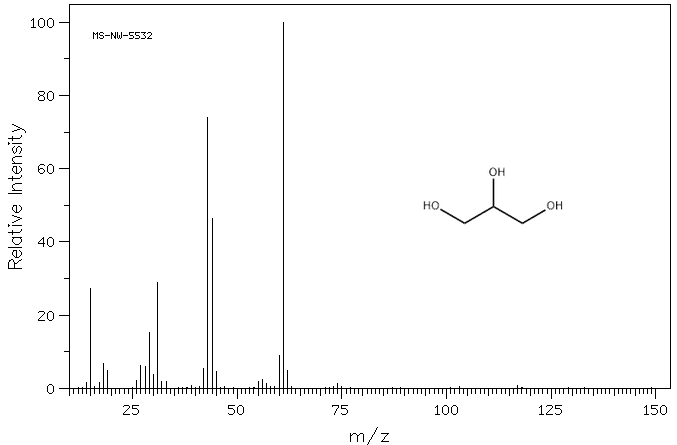
\includegraphics[width = 0.7\linewidth]{Images/ms_glycerol.png}
   	 \caption{Spectre MS du Glycérol}
   	 \label{fig:ms_glycerol}
    \end{figure}
    
    Pour pouvoir le faire on utilise une machine spécialisée appelée spectromètre de masse qui contient généralement :
    \begin{itemize}
   	 \item un tube de liquide : dans lequel on introduit l'élément chimique
   	 \item un ioniseur : qui par le biais de faisceau d'électrons permet d'ioniser l'élément
   	 \item un accélérateur de particules : qui a pour but de dévier les radicaux d'un rayon de courbure qui dépend de leur masse sur charge
   	 \item un détecteur : qui permet d'évaluer ces rayons de courbure (par conséquent les masses sur charge) et d'avoir les abondances de ces radicaux (ou encore intensité)
    \end{itemize}
    
    On parle ainsi de :
    \begin{itemize}
   	 \item Spectrométrie de masse à haute résolution \acrshort{HRMS}:
   	 lorsqu'on utilise des spectromètres de masse spécialisés tels que \textbf{Orbitrap}.
   	 \item Chromatographie liquide/ Spectrométrie de masse \textbf{LC/MS}:
   	 lorsqu'on utilise la technique de séparation de molécules contenues dans une solution aqueuse nommée chromographie avant la spectrométrie de masse  
   	 \item Spectrométrie \textbf{$MS^{2}$} (MS/MS) :
   	 lorsqu'on utilise des spectromètres de masse qui possèdent deux étapes d'ionisation consécutives avant analysation
    \end{itemize}

    \subsubsection{Spectrométrie RMN}

    Cette méthode de spectrométrie a plutôt pour but d'extraire d'un élément chimique, les déplacements chimiques et les intensités d'excitation que réalisent ses atomes de types spécifiques (Hydrogène, Carbone etc \dots), lorsqu'il est placé dans un champ magnétique (zone de forces issues d'un aimant ou de déplacements d'électrons).
    Ces informations constituent ce qu'on appelle un spectre de résonnance magnétique nucléaire ou encore spectre  \acrshort{RMN}, qu'on visualise généralement sur un graphique semblabe à celui de la Figure \ref{fig:hrmn_glycerol} \footnote{Prise sur \href{https://www.chemicalbook.com/SpectrumEN_56-81-5_Raman.htm}{https://www.chemicalbook.com/SpectrumEN\_56-81-5\_Raman.htm}} étant celui du glycérol.

    \begin{figure}
   	 \centering
   	 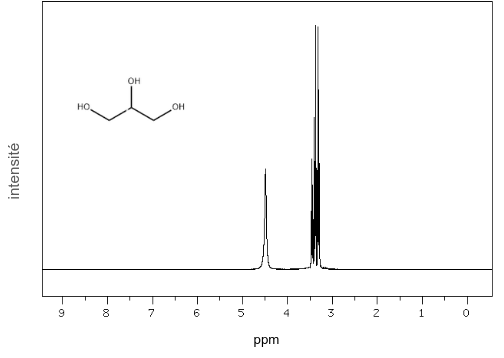
\includegraphics[width = 0.7\linewidth]{Images/hrmn_glycerol.png}
   	 \caption{Spectre RMN du Glycérol observant les atomes d'hydrogène}
   	 \label{fig:hrmn_glycerol}
    \end{figure}

    Pour obtenir ces informations, on utilise un spectromètre  \acrshort{RMN} encore appelé sonde RMN, qui est un compartiment qui permet d'utiliser des champs magnétiques excitant des types d'atomes précis d'une molécule, en considérant un champ de base (celui agissant sur le Tetramethylsilane TMS).

	 Lorsqu'on observe 'n' types d'atomes on parle de spectrométrie 'n-RMN', par exemple pour:
   	 \begin{itemize}
   		 \item la spectrométrie \textbf{1-RMN} : on a la spectrométrie sur hydrogène (H-RMN), Spectrométrie sur carbone (C-RMN)
   		 \item la spectrométrie \textbf{2-RMN} : on a  \acrfull{TOCSY} qui observe les croisements hydrogène-hydrogène), \acrfull{HSQC} qui observe les croisements hydrogène-carbone
   	 \end{itemize}

    Ces techniques permettent d'avoir des informations sur des molécules sans pour autant avoir leurs structures, qui en laboratoire est un processus long surtout pour la découverte de médicaments basée sur les produits naturels.
    Ils sont très utiles dans ce processus car ils permettent d'éviter de réaliser des expérimentations sur des molécules déjà identifiées en observant les correspondances de spectres entre molécules. On appelle cette opération la déréplication.
    
    \subsection{Déréplication et réseau moléculaire}

   	 La \textbf{déréplication} est une opération qui consiste à trouver dans un ensemble de molécules, celles qui ont déjà été identifiées par correspondance de spectres par rapport à celles identifiées et sauvegardées dans des bases de données.
   	 Elle permet de réduire les expérimentations d'essais - erreurs en donnant la possibilité de se concentrer sur des molécules inconnues.
   	 Dans le but de retrouver ces molécules inconnues, on observe leurs correspondances avec ceux qui ont été identifiées pour essayer de détecter les synergies et relations qui peuvent exister entre elles.
  	 
   	 Pour bien le visualiser, on utilise un graphe où un nœud correspond à une molécule (représentée par un spectre), avec une liaison entre deux nœuds correspondant au niveau de ressemblance (similarité) ou de différence entre eux.
   	 Il faut noter que ces nœuds ou encore sommets portent les métadonnées disponibles de leurs molécules correspondantes.
   	 On appelle ce type de graphe un \textbf{réseau moléculaire}, qui plus formellement est un graphe epsilon-voisinage, avec des sommets étant des molécules et des arêtes correspondant à la similarité ou la dissimilarité entre leurs spectres (\acrshort{MS} ou \acrshort{RMN}).
  	 
   	 Plus ce réseau contient de molécules identifiées, plus on augmente les possibilités d'identifier toutes les molécules y contenues par des restrictions d'expérimentation.
   	 On parle ainsi de \textbf{réseau identifié} quand toutes les molécules y contenues sont identifiées.
   	 Cela signifie que bien construire un réseau moléculaire (par le choix de métrique et des liaisons) permet d'accélérer le processus de découverte.
   	 Des différents moyens d'en construire et du type de spectre utilisé, il existe plusieurs outils ou méthodes dont les plus communs sont \acrfull{GNPS} et \acrfull{MADByTE}.
  	 
   	 \subsubsection{\acrfull{GNPS}}
  	 
   	 \textbf{GNPS} \cite{wang2016sharing} est une plateforme dont le processus principal prend en entrée des spectres MS de molécules pour construire le réseau moléculaire.
   	 Comme on peut le voir sur la Figure \ref{fig:gnps3}, ce processus suit plusieurs étapes:
  	 
   	 \begin{figure}
   		 \begin{center}
       		 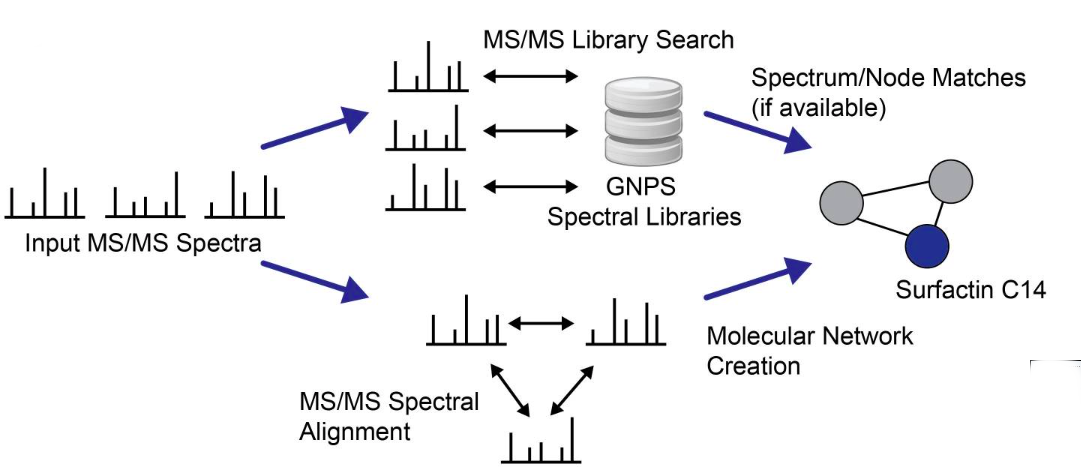
\includegraphics[width = 0.7\textwidth]{Images/GNPS4.png}
   		 \end{center}
   		 \caption{Processus de GNPS \cite{wang2016sharing}}
   		 \label{fig:gnps3}
   	 \end{figure}

   	 \begin{itemize}
   		 \item \textbf{Construction du template du réseau des molécules d'entrées} : cette étape a pour objectif de construire le réseau des molécules d'entrées en utilisant comme mesure de similarité le cosinus de similarité avec un seuil donné (plus de 0.63 en pratique)
   		 \item \textbf{Identification des molécules par correspondance dans sa base de données}  : cette étape à pour objectif de trouver les molécules d'entrées qui sont déjà dans la base de données, en faisant une recherche basée sur la correspondance de spectres utilisant le cosinus de similarité et également un seuil donné (plus de 0.7 en pratique)
   		 \item \textbf{Attachement des méta-données au template précédent}: cette étape visent à ajouter les informations des molécules identifiées et non identifiées sur leurs sommets respectifs du graphe.
   	 \end{itemize}

   	 Il faut noter que chacune des valeurs de seuil de similarité utilisées ont des significations particulières pour les biologistes. Si le seuil a une valeur supérieure à 0.7 alors on cherche des correspondances exactes, si par contre, on a une valeur comprise entre 0.63 à 0.7, on cherche des correspondances pour exploration.
  	 
   	 \subsubsection{\acrfull{MADByTE}}

   	 \textbf{MADByTE} est également un outil qui permet de construire le réseau moléculaire correspondant à un ensemble de spectres de molécules; il prend en entrée les spectres HSQC et TOCSY des molécules.
   	 Le réseau est tout de même différent qu'avec celui de GNPS, car on retrouve un nouveau type de nœud associé à un système de spin.
  	 Un système de spin est un ensemble de déplacements chimiques considérés comme identiques par tolérance.
   	 De ce fait, une molécule peut être vue comme un ensemble de systèmes de spins qu'il contient, et à cet effet son sommet est relié à tous ceux de ses systèmes de spins d'une similarité complète.

   	 Comme on peut le voir sur la Figure \ref{fig:madbyte}, ils suit les étapes suivantes:
   	 \begin{itemize}
   		 \item \textbf{Prétraitement des spectres \acrshort{HSQC} et \acrshort{TOCSY}} : cette étape vise à supprimer les déplacements considérés comme inutiles, en tenant compte des solvants qui ont été utilisés pour acquérir les spectres et en s'assurant qu'après suppression les spectres TOCSY soient toujours symétriques

   		 \item \textbf{Croisement des spectres TOCSY et HSQC obtenus} : cette étape vise à conserver les déplacements qui se correspondent par rapport aux atomes d'hydrogènes pour chacun des couples de spectres

   		 \item \textbf{Calcul des système de spins} : cette étape vise à regrouper les déplacements identiques que sont les systèmes de spins avec des marges d'erreur donnés pour les atomes d'hydrogène et de carbone

   		 \item \textbf{Construction du réseau}: cette étape vise à construire le réseau de molécules.
   		 On calcule les similarités entre les systèmes de spins en utilisant l'indice de Jaccard.
   		 Il faut aussi noter que chaque sommet d'une molécule sera lié aux sommets de tous ses systèmes de spins d'une valeur de similarité complète (valeur 1)
   	 \end{itemize}

   	 \begin{figure}
   		 \begin{center}
       		 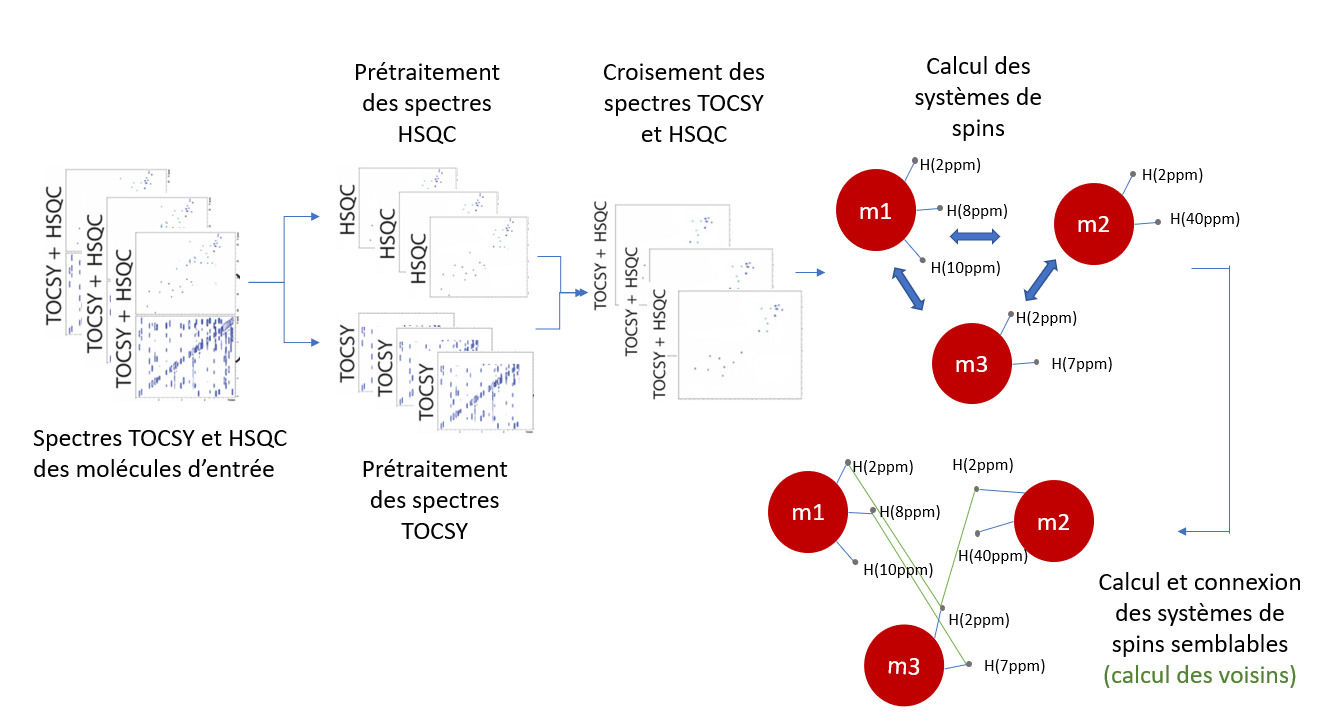
\includegraphics[width = 0.7\textwidth]{Images/madbyte.png}
   		 \end{center}
   		 \caption{Processus de MADByTE}
   		 \label{fig:madbyte}
   	 \end{figure}

   	 On obtient un réseau qui, pour des raisons de lisibilité peut être simplifié en supprimant les sommets de systèmes de spins qui ne sont liés à aucun autre système.
   	 On obtient un \textbf{réseau d'association} qui peut encore être plus lisible en considérant les sommets de systèmes de spins connectés comme un sommet.

   	 Nous remarquons que l'on utilise un réseau moléculaire parce qu'il permet d'explorer des liaisons entre les molécules, tout en regroupant les molécules ou encore spectres similaires dans des groupes ou encore clusters qui se forment naturellement.
   	 Ces groupes qu'on retrouvent permettent par le biais d'observations et d'analyse des spectres, et des structures des molécules identifiées, d'avoir des orientations d'expérimentations.
   	 De ce fait les algorithmes comme GNPS et MADByTE regroupent des spectres de molécules les plus semblables, ce qui se rapproche très clairement du clustering.

\section{Plan du mémoire}

Le reste de ce mémoire est organisé comme suit.
Le Chapitre 2 présente %les bases nécessaires à la compréhension du travail, allant des notions d'atomes et molécules aux réseaux moléculaires. Il se termine par
une revue de littérature des méthodes de clustering, de clustering multi-vues et d’ensemble de clustering utiles à la résolution du problème.
Dans le Chapitre 3, nous détaillons les méthodes proposées.
Le Chapitre 4 présente nos expérimentations et les résultats obtenus.
Enfin, le Chapitre 5 conclut ce document en résumant les principaux résultats et en discutant des implications futures de notre recherche.


    \chapter{État de l'art}

    \section{Clustering}
  	  Le \textbf{clustering} est un processus d'analyse exploratoire qui consiste sur la base d’un ensemble de données, à regrouper ceux qui sont les plus similaires entre eux et d'en éloigner ceux qui le sont moins.
  	  Cette opération de regroupement amène à obtenir des groupes d’observations appelés clusters dans lesquels se trouvent des observations qui sont les plus similaires les unes, des autres.
      
  	  Plusieurs approches de construction de clusters ou de regroupement d’observations ont vue le jour, ce qui a conduit à la création de divers algorithmes de clustering, qui peuvent être regroupés comme suit:

  	  \begin{itemize}
  		  \item \textbf{Clustering par partitionnement}: on cherche à construire des clusters qui seront disjoints entre eux et dont séparés, ce qui conduit à partitionner ou encore à diviser l’ensemble des observations. Les plus communs de ce type d’algorithmes sont l'algorithme KMEANS et l'algorithme de clustering spectral.
     	 
  		  \item \textbf{Clustering hiérarchique}: L’approche est de construire une hiérarchie de clusters des données, de façon ascendante ou descendante. Ascendante selon le fait qu’on débute la construction depuis chaque observation, et descendante en revanche en partant de tout l’ensemble des observations. Comme algorithmes les plus utilisés, on a les algorithmes \acrfull{CAH} et \acrfull{CDH}.
    
  		  \item \textbf{Clustering par modélisation} : l’idée est de construire des clusters qui seront modélisés d’une façon donnée. Communément les clusters sont modélisés par des modèles probabilistes, ce qui est le cas pour l’algorithme \acrfull{GMM}.
    
  		  \item \textbf{Clustering par densité} : L’approche est celle d’identifier une zone d’observations à forte densité comme étant un cluster d’observations. L'algorithme \acrfull{DBSCAN} étant le plus populaire, avec des versions prenant des graphes non pondérés et planaires tels que l'algorithme \acrfull{SCAN} et \acrfull{NS-DBSCAN}.
     	 
  	  \end{itemize}
    
  	  Les données spectrales telles que les spectres MS et RMN pouvant être impactées respectivement par la qualité de l’ionisation et des matériaux utilisés, peuvent avoir des bruits.
  	  De plus, les biologistes détectent les clusters dans les réseaux moléculaires en les considérant naturellement par des zones à densité relativement forte.
  	  De ce fait, utiliser des algorithmes de clustering par modélisation ou par densité sur de telles données est logique car ils ont principalement la propriété d'être résistants aux bruits.
  	  Nous parlerons ainsi par la suite, plus spécifiquement des algorithmes DBSCAN et ses versions pour les graphes SCAN et NS-DBSCAN.
    
 			 
  	  \subsection{ \acrfull{DBSCAN}}
     	 
     	   \textbf{DBSCAN} %\cite{khan2014dbscan}
           est un algorithme de clustering utilisé pour regrouper des points de données similaires en définissant un cluster comme une zone à grande densité.
  	 
     	   Soit $N(x, \epsilon)$ l'ensemble des observations voisines de l'observation $x$ étant dans le rayon $\epsilon$, on a :
     	   \begin{equation}
     		   N(x, \epsilon) = \{ x' | d(x', x) \leq \epsilon\}
     	   \end{equation}
		 
     	   L'algorithme retrouve ces zones progressivement par parcours en largeur, grâce à des points d'intérêts qu'on peut voir à la Figure \ref{fig:mod_dbscan} qui sont:
     	   \begin{itemize}
				   \item \textbf{Core Point} : observation caractérisée par le fait que le nombre de ses voisins dépasse le seuil de densité minimum $MinPts$
				   \item \textbf{Border Point} : observation appartenant au voisinage d'un \textbf{Core Point} mais ne l'est pas
				   \item \textbf{Noise Point} : est une observation qui n'est ni \textbf{Core Point}, ni \textbf{Border Point} c'est à dire du bruit
     	   \end{itemize}
      
     	   \begin{figure}
				   \centering
				   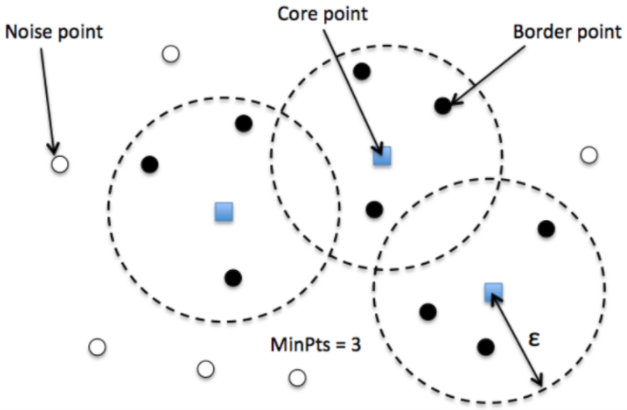
\includegraphics[width=0.5\linewidth]{Images/dbscan.png}
				   \caption{Types clés d'observations de DBSCAN}
				   \label{fig:mod_dbscan}
		   	\end{figure}
      
  		  Des versions \cite{bhattacharjee2021survey} de cet algorithme ont été mis en place dans le but de réduire son temps de calcul, de réduire l'impact de ses paramètres de densité sur la construction des clusters, et de prendre en compte de différentes natures des données d'entrée (image, texte, graphe, \dots).
  		  On retrouve ainsi des algorithmes tels que SCAN et NS-DBSCAN qui permettent de prendre des graphes non pondérés en entrée et planaires respectivement.
     	 
  	  \subsection{\acrfull{SCAN}}
      
  		  \textbf{SCAN} %\cite{xu2007scan, shiokawa2018scalescan}
          \cite{shiokawa2018scalescan} est un algorithme de partitionnement de graphe non pondéré, ayant pour objectif de construire les groupes de sommets, en les voyant comme des zones à forte densité de sommets.
  		  L'algorithme calcule premièrement pour chaque sommet du graphe l'ensemble de ses voisins (qui constitue sa structure), puis utilise l'algorithme DBSCAN avec pour mesure de similarité la distance cosinus.
  	 
  	  \subsection{\acrfull{NS-DBSCAN}}
    
  		  \textbf{NS-DBSCAN} \cite{wang2019ns} est un algorithme de partitionnement de graphe planaire, qui a pour but de regrouper les sommets qui y sont contenus, en considérant ces groupes comme des zones à forte densité de sommets.
  		  L'algorithme utilise l'algorithme DBSCAN en considérant les sommets du graphe comme des observations et en utilisant comme distance entre sommets l'algorithme LSPD \cite{wang2019ns} (Local Shortest Path Distance).
    
  		  Malgré le fait que ces deux précédents algorithmes prennent en entrée des graphes d'observations, ils ne tiennent pas compte des spécificités des réseaux moléculaires qui contiennent déjà les densités de voisinage.

	\section{Clustering Multi-vues}

	Le clustering multi-vues est une technique d'apprentissage non supervisée qui consiste à regrouper des observations similaires entre eux et d'en éloigner ceux qui ne le sont pas, en tenant compte du fait qu'on utilise pour chaque observation plusieurs représentations différentes appelées vues.
    
	Le clustering multi-vues se différencie du "clustering" principalement par le fait qu'on cherche à exploiter la complémentarité et le consensus entre des vues de données dans le but de mieux les regrouper.
	La complémentarité et le consensus entre les vues sont donc des notions importantes à définir:
	\begin{itemize}
  	  \item \textbf{Complémentarité} : la complémentarité entre deux vues V1 et V2 est décrit par le fait qu'il existe sur des observations, des informations qui ne peuvent être représentées que par V1 et d'autres que par V2
  	  \item \textbf{Consensus}: le consensus entre deux vues V1 et V2 est décrit par le fait qu'il existe sur des observations, des informations qui sont décrites par V1 et par V2 simultanément
	\end{itemize}

	En considérant une dataset $X$ avec deux vues $X^1$ et $X^2$, Daguplaet et al. \cite{dasgupta2001pac}
    ont démontré que la probabilité d'erreur issue du conflit des hypothèses (prédicteurs) $f_1$ et $f_2$ sur les vues $X^1$ et $X^2$ respectivement, est supérieure ou égale aux probabilités faites par $f^1$ ou $f^2$ sur ces mêmes vues.
    D'où minimiser le désaccord entre $f^1$ et $f^2$ sur les vues, permet de réduire les erreurs de $f^1$ et $f^2$ simultanément.
    
    Cela a permis d'avoir les principes suivants qui constituent la base des algorithmes de clustering multi-vues:
	\begin{itemize}
  	  \item \textbf{Principe associé à la complémentarité}: les vues doivent être utilisées afin de décrire les observations de manière plus complète et plus précise.
  	  \item \textbf{Principe associé au consensus}: il faut maximiser le consensus ou encore la cohérence entre les vues des observations afin de mieux cerner les informations complémentaires entre les vues
	\end{itemize}
    
	La mise en œuvre de ses principes a conduit à l'obtention des branches d'algorithmes tel qu'on peut le voir sur la Figure \ref{fig:typo-mvc}: ceux qui apprennent des représentations globales des différentes vues des données et ceux qui ne le font pas.
    \begin{figure}
        \centering
        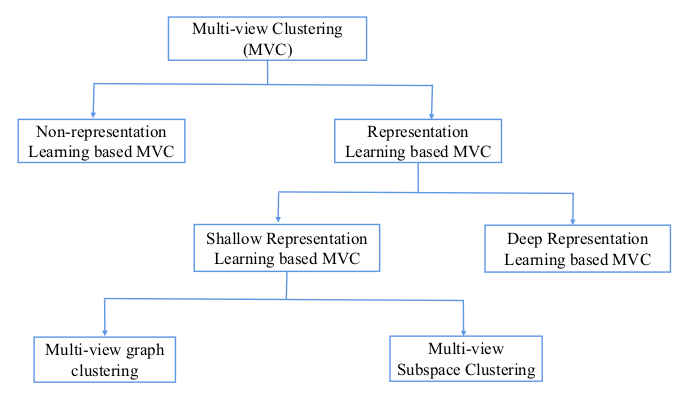
\includegraphics[width= 0.6\linewidth]{Images/taxonomyMultiViewClustering.png}
        \caption{Taxonomie des algorithmes de clustering multi-vues \cite{chen2022representation}}
        \label{fig:typo-mvc}
    \end{figure}

	\subsection{Algorithmes sans apprentissage de représentation}

  		  \subsubsection{Algorithmes de co-formation}
     	 
  		   Ces algorithmes cherchent à maximiser l'accord entre les vues tout en améliorant itérativement les clusters allant d'une vue à l'autre.
  		  On construit initialement les clusters pour chaque vue, et les clusters d'une vue sont améliorés en utilisant ceux des autres vues dans le but de maximiser le consensus d'observations entre eux.
  		  On procède ainsi tour à tour un certain nombre d'itérations (Figure \ref{fig:co-train1}) pour chaque vue. On peut trouver les algorithmes de co-formation \cite{bickel2004multi} adaptant les algorithmes \acrshort{EM}, \acrshort{CAH} et KMEANS Sphérique %\cite{dhillon2001concept}
          .
		 
     	   \begin{figure}
     		   \centering
     		   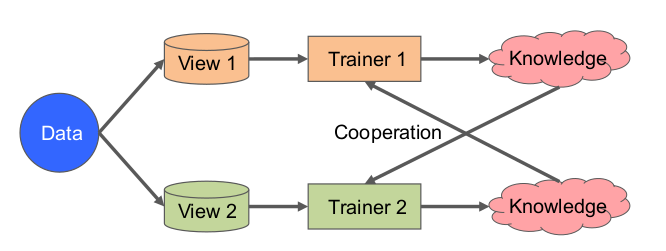
\includegraphics[width=0.6\linewidth]{Images/co-training.png}
     		   \caption{Processus général des algorithmes de clustering multi-vues de co-formation \cite{yang2018multi}}
     		   \label{fig:co-train1}
     	   \end{figure}
     	   % On peut dès lors comprendre que ces algorithmes possèdent un défaut majeur qui est le temps d'exécution, car on reconstruit les clusters en un certain nombre d'itérations.
    
  	  \subsubsection{Algorithmes multi-noyaux}
     	   S'il est difficile de construire des clusters dans un espace d'une dimension donnée, on pourrait plus aisément le faire en projetant les observations dans un espace correspondant de plus grande dimension.
  		  C'est sur ce principe que les algorithmes de clustering par noyaux sont construits. On recherche une fonction noyau qui permettra d'obtenir de meilleurs clusters suivant un critère d'évaluation comme l'inertie intra-classe.
     	   Cette fonction noyau agglomère les espaces des données différentes vues, en combinant linéairement ou non des fonctions noyaux obtenues sur chacune des vues (voir la Figure \ref{fig:multi-kernel1}). On peut citer l’algorithme multi-noyau auto-pondéré \cite{yang2018multi} qui adapte KMEANS en modifiant la définition de l’inertie intraclasse avec une fonction noyau gaussienne pondérée.
    
  			  \begin{figure}
      			  \centering
      			  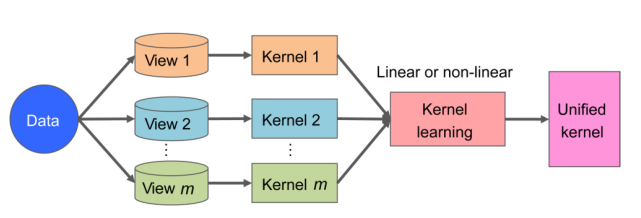
\includegraphics[width = 0.6\linewidth]{Images/multi-kernel.png}
      			  \caption{Processus général des algorithmes de clustering multi-vues multi-noyaux \cite{yang2018multi}}
           		 \label{fig:multi-kernel1}
  			  \end{figure}

  		  \item \textbf{Algorithmes de factorisation matricielle}
     	 
  		  Ils sont utilisés pour le problème de clustering multi-vues en factorisant les matrices de données des vues (non négatives) en des couples de matrices dit facteurs.
  		  Pour chacun de ces couples, on a l'un qui représente la pondération liée à une vue précise et l'autre l'indicateur des clusters pour cette même vue.
  		  Cet indicateur contenant de nouveaux vecteurs représentatifs d'observations très similaires pour ceux d'un même cluster et peu similaires pour ceux ne l'étant pas.
		 
     	   L'indicateur global des clusters est ainsi calculé par agglomération de chacune des vues par consensus.
  		  Plus formellement, on a le problème d'optimisation de l'équation \ref{equa:nmf}, où $U^{(v)}$ désigne la matrice de poids de la vue $v$, $C^{(v)}$ l'indicateur de la vue $v$, $C^*$ est l'indicateur globale et $\Phi$ est une fonction de différence de $C^*$ et $C^{(v)}$.
  		  Il faut noter que $||A||_{F}^{2} = tr(A.A^{T}) = \sum_{i,j} a_{i,j}^2$

     	   \begin{equation}
  			   \begin{aligned}
 				   \min {\sum_{v=1}^{V} {|| X^{(v)} - U^{(v)}.C^{(v)} ||}_F^2 + \Phi(C^{(v)}, C^{*})} \\
 				   \text{s.t, $U^{(v)},C^{(v)},C^{*} \geq 0$,}
     		   \end{aligned}
     		   \label{equa:nmf}
     	   \end{equation}

  	  \subsubsection{Algorithmes spectraux}
     	 
  		  Effectuer du clustering revient à trouver k groupes d'observations similaires entre eux. Cela se fait par une fonction $f$ qui permet d'attribuer à chaque observation un indicateur propre à un des $K$ clusters. On peut ainsi voir que $f$ est lui-même un indicateur pour attribuer une observation à un cluster donné et peut être vu comme une projection d'observations où les vecteurs appartenant au même cluster se ressemblent fortement et non pour ceux de clusters différents.
     	 
  		  L'objectif de ces algorithmes est de calculer $f$, tout en tenant compte des similarités entre couple d'observations (on revient à un graphe de similarité) pour chacune des vues.
  		  Plus formellement on cherche à résoudre le problème d'optimisation \ref{equa:spectral3} où $L_{v}$ est le laplacien du graphe de similarité des observations dans la vue $v$, $\alpha_{v}$ l'importance attribué à la vue $v$.
     	 
  		  \begin{equation}
  			  \begin{aligned}
      			  \min_{F^{T}F = I, \alpha} \sum_{v} tr(F^{T} L_v F) \\
      			  \text{s.t, } \sum_{v} \alpha_{v} = 1 \text{ , } \alpha_{v} \geq 0
  			  \end{aligned}
  			  \label{equa:spectral3}
  		  \end{equation}
  		  La contrainte $F^{T}F = I$ permet de s'assurer que les nouvelles dimensions ne se corréleront pas.
  		  % Les vecteurs propres dans l'ordre croissant de leurs valeurs propres du laplacien conjugué $L$ seront calculés, puis soumis à un algorithme de clustering classique pour pouvoir trouver $F$. Il faut noter qu'avec cette méthode de clustering, il est possible de détecter le nombre de clusters approprié (qui est le nombre de vecteurs propres), en s'appuyant sur les écarts entre les valeurs propres consécutives. Le nombre $K$ de clusters peut être choisi ou obtenu en détectant une grande variation entre deux valeurs propres consécutives selon l'ordre croissant de ces valeurs.


    \subsection{Algorithmes basés sur l'apprentissage de représentation}
 
        %Dans cette catégorie d'algorithmes, on a ceux qui utilisent les réseaux de neurones pour construire les représentations (on parle de "Deep representation learning-based MVC" en anglais) et d'autres qui ne les utilisent pas (on parle de "Shallow representation learning-based MVC" en anglais) dit d'algorithmes peu profond.

  	  \subsubsection{Algorithmes basés sur les graphes}
		 
     	   Pour pouvoir tenir compte des données à plusieurs vues, ils construisent pour chaque vue des graphes de similarités, puis définissent une politique de fusion de ces graphes, qui s'appuie généralement sur l'attribution des poids à des observations par rapport aux groupes formés.
  		  De là on obtient un graphe unifié ou global de similarité qui pourra être sujet de partitionnement pour obtenir les clusters.
  		  On cherchera ainsi à trouver les poids amenant à avoir le moins d'erreurs possible de fusion des vues.
  		  On peut ainsi retrouver l'algorithme \acrfull{MVGL} \cite{zhan2017graph} qui met en œuvre ce principe.
    
     	   \begin{figure}
     		   \centering
    			  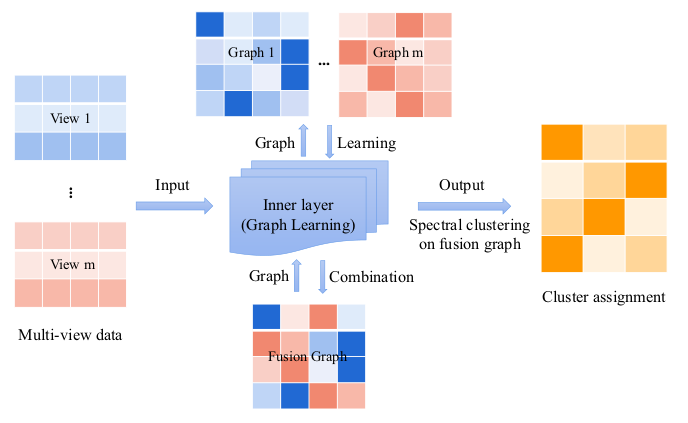
\includegraphics[width=0.75\linewidth]{Images/graph2.png}
     		   \caption{Processus général des algorithmes de clustering multi-vues basés sur les graphes \cite{chen2022representation}}
     		   \label{fig:graph1}
     	   \end{figure}

     	   Plus formellement le problème d'optimisation générale est celui de l'équation \ref{equa:graph1}, où $A^{(v)}$ est la matrice de similarité spécifique à la vue $v$, $S$ représente la matrice de similarité du graphe unifié, $Dis$ pour la similarité ou la dissimilarité utilisée dans les vues, et $\Phi$ est une fonction d'erreur de fusion de $S$ et $A^{(v)}$.

     	   \begin{equation}
  			   \begin{aligned}
 				   \min {\sum_{v=1}^{V} \sum_{i \neq j}^{n} \text{Dis}(X_i^{(v)}, X_j^{(v)})A^{(v)} + \Phi(A^{(v)}, S)} \\
 				   \text{s.t, $A^{(v)},S \geq 0$,}
     		   \end{aligned}
     		   \label{equa:graph1}
     	   \end{equation}
  	 

  	  \subsubsection{Algorithmes de sous-espaces}
		 
     	   L'idée ici est de rechercher une représentation unifiée des vues pour chaque observation, puis d'utiliser un algorithme de clustering dessus pour obtenir les clusters.
  		  De ce fait, on procède généralement de deux manières tel que sur la Figure \ref{fig:subspace}:
     	 
     	   \begin{enumerate}
     		   \item soit on apprend directement la représentation depuis les sous-espaces des vues des données
     		   \item soit on apprend la représentation globale sur un espace latent issus de ses sous espaces des vues
     	   \end{enumerate}

  		  Il faut noter que chaque sous espace des vues est généralement obtenue par réduction de dimension des données de ces dernières.

     	   \begin{figure}
     		   \centering
     		   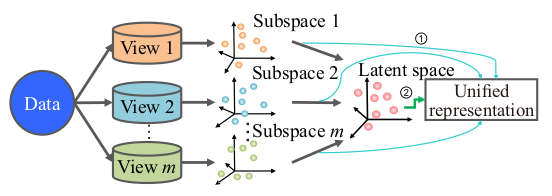
\includegraphics[width = 0.6\linewidth]{Images/subspace.png}
     		   \caption{Processus général des algorithmes de clustering multi-vues de sous-espaces \cite{yang2018multi}}
     		   \label{fig:subspace}
     	   \end{figure}
     	 
  		  On peut citer l'algorithme \acrfull{MCLES} \cite{mcles} qui est la base des algorithmes les plus performants de ce type.
     	 
        \subsubsection{Algorithmes basés sur l'apprentissage profond de représentation}
     	 
   	  Dans le but d'explorer complètement les espaces de données originaux pour construire une représentation unifiée, ces algorithmes utilisent des réseaux de neurones au vue de leur performance sur des problèmes supervisés.
  		  Comme le modèle d'auto-encodage \cite{wang2016auto} utilisé dans le domaine du traitement du langage naturel, ces réseaux sont entraînés par rétropropagation des erreurs liées aux regroupements effectués sur les représentations obtenues des observations.
  		  La Figure \ref{fig:deepLearning} illustre très bien le processus général de ces algorithmes.

     	   \begin{figure}
     		   \centering
     		   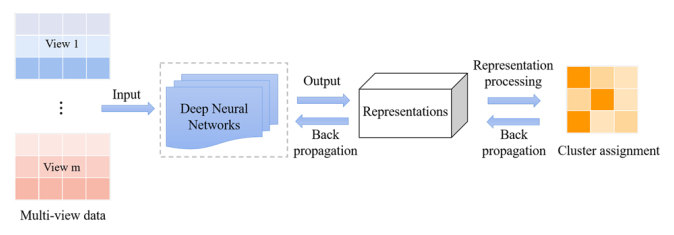
\includegraphics[width = 0.75\linewidth]{Images/multiviewCLusteringDeep.png}
     		   \caption{Processus général des algorithmes de clustering multi-vues d'apprentissage profond de représentation \cite{chen2022representation}}
     		   \label{fig:deepLearning}
     	   \end{figure}

  	  \subsection{Comparaison des algorithmes de clustering multi-vues}

  	  Nous avons le Tableau \ref{tab:comp_multivues} de comparaison suivant mettant en évidence les avantages et limites des algorithmes en se basant sur leurs propriétés.
        
        %\vspace*{20mm}
        \clearpage % ou \newpage
        
  	  \begin{longtable}{|p{4.5cm}|p{6cm}|p{6cm}|}
  		  \caption{Tableau de comparaison des algorithmes de clustering multi-vues}
  		  \label{tab:comp_multivues}
  			  \hline
 				   \textbf{Algorithmes} & \textbf{Avantages} & \textbf{Limites} \\
  			  \hline
     				   Algorithmes de co-formation
     				   &
     				   {- ils améliorent itérativement et simultanément les clusters de chaque vue} \newline\newline
     				   {- ils permettent d’obtenir des regroupements ”optimaux” dans chacune des vues}
     				   &
     				   {- ils reconstruisent les clusters à chaque étape, ce qui peut alourdir le temps de calcul des clusters optimaux}
     				   \\
     				   \hline
     				   Algorithmes multi-noyaux
     				   &
     				   {- ils permettent d'obtenir des clusters globaux dans un espace unifié de plus grande dimension (sans l'obtenir analytiquement) permettant d'obtenir les meilleurs regroupements } \newline\newline
     				   {- ils permettent de mettre une nouvelle observation dans un cluster sans pour autant relancer tout le processus} \newline\newline
     				   {- ils sont peu sensibles aux bruits}
     				   &
     				   {- on ne peut pas obtenir l'espace de plus grande dimension cible} \newline\newline
     				   {- ils dépendent fortement du choix de la fonction noyau unifiée (de la fusion des noyaux de chaque vue)}
     				   \\
  			  \hline
     				   Algorithmes spectraux
     				   &
     				   {- ils permettent d'obtenir un indicateur unifié des clusters tout en calculant et intégrant les importances des vues dans la construction des clusters}
     				   &
     				   {- l'attribution d'une nouvelle observation à un cluster nécessite un ré-apprentissage des paramètres} \newline\newline
          			  {- ils sont sensibles aux bruits} \newline\newline
     				   {- ils dépendent généralement de métriques de similarité spécifiques pour la construction des matrices de similarité, ce qui le rend instable } \newline\newline
     				   {- ils se basent uniquement sur les données des vues complètes}
     				   \\
  			  \hline
     				   Algorithmes de factorisation
     				   &
     				   {- ils permettent d'obtenir un indicateur unifié des clusters et des indicateurs spécifiques pour chacune des vues, tout en évaluant l'importance de ces vues dans les regroupements} \newline\newline
     				   &
     				   {- l'attribution d'une nouvelle observation à un cluster nécessite un ré-apprentissage des paramètres}
     				   \\
  			  \hline
     				   Algorithmes basées sur les graphes
     				   &
     				   {- ils permettent d'obtenir un graphe de similarité globale utile à l'exploration des données} \newline\newline
     				   {- ils sont peu sensibles aux bruits} \newline\newline
     				   {- ils permettent de réduire la dimensionnalité des données de chaques vues}
     				   &
     				   {- l'attribution d'une nouvelle observation à un cluster nécessite un ré-apprentissage des paramètres} \newline\newline
     				   {- ils dépendent généralement de métriques de dissimilarité et de similarité}
     				   \\
  			  \hline
     				   Algorithmes de sous-espaces
     				   &
     				   {- ils permettent d'obtenir une représentation globale des vues tout en optimisant les regroupements } \newline\newline
          			  {- ils permettent de réduire la dimensionnalité des données d'origine } \newline\newline
     				   {- ils sont peu sensibles aux bruits}
     				   &
     				   {- l'attribution d'une nouvelle observation à un cluster nécessite un ré-apprentissage des paramètres}
     				   \\
  			  \hline
     				   Algorithmes basés sur l'apprentissage profond de représentation
     				   &
     				   {- ils permettent d'obtenir une représentation unifiée des vues } \newline\newline
     				   {- l'attribution d'une nouvelle observation ne nécessite pas forcément un ré-apprentissage des paramètres}
     				   &
     				   {- on a le problème d'explicabilité du réseau}
     				   \\
  			  \hline
  		  \end{longtable}
  		  
     		 
  	  Au vue de cette analyse, les algorithmes de graphes et de sous espace sont ceux qui correspondent le plus à notre problème.
  	  Cela parce qu'ils sont résistants aux bruits ce qui est souhaitable vu que les données spectrales en contiennent.
  	  De plus les réseaux moléculaires étant des graphes de similarité, ils peuvent être utilisés dans les algorithmes de graphes; et les algorithmes de sous espaces peuvent combiner des spectres de molécules en un seul (ce qui a fait partie d'une des idées initiales).
  	  Nous développons dans les sections qui suivent les algorithmes \acrshort{MCLES} et \acrshort{MVGL} qui font partie des plus performants de ces catégories.

  	  \subsection{\acrfull{MCLES}}

  	  L'idée ici est de construire une représentation unifiée (une nouvelle représentation combinée des vues) dans un espace latent, afin de calculer une matrice de similarité de cette représentation qui sera utilisée pour effectuer les regroupements.
  	  Cela dit, en entrée on a les données des vues et le nombre voulu de clusters, pour avoir en sortie la représentation unifiée, les indicateurs de clusters des observations et les clusters après utilisant de l'algorithme KMEANS.
  	  Comme la Figure \ref{fig:mcles1} le montre on calcule d'abord la représentation unifiée, puis la matrice de similarité et enfin les indicateurs de clusters d'observations itérativement jusqu'à ce qu'on obtienne le meilleur clustering possible ou après un certains nombre d'itérations.
   
  	  \begin{figure}
			\centering
			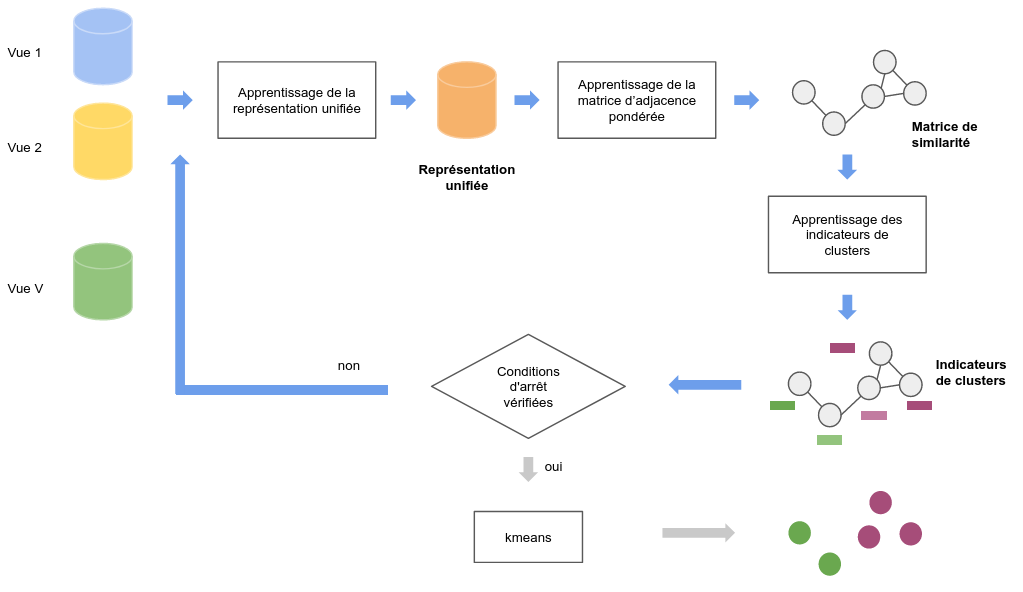
\includegraphics[width = \linewidth]{Images/mcles1.png}
			\caption{Processus de l'algorithme MCLES}
			\label{fig:mcles1}
  	  \end{figure}
    
   	 En supposant que la représentation unifiée d'une observation le décrit pleinement, on peut retrouver sa représentation pour une vue, en appliquant sur cette représentation unifiée une tâche donnée qui peut être une pondération (projection).
  	  Plus formellement pour l'observation $i$, on a $x_i^{(v)}$ son vecteur caractéristique dans la vue $v$, $h_i$ étant sa représentation unifiée et $W^{(v)}$ étant la matrice des poids de la vue $v$.
  	  \begin{equation*}
			x_i^{(v)} = W^{(v)} h_i
  	  \end{equation*}
  	  En considérant que les observations sont des colonnes de matrices de données des vues, on obtient l'expression suivante
  	  \begin{equation*}
			X = WH \text{ où } X = \begin{pmatrix} X^{(1)}\\X^{(2)}\\\vdots\\X^{(V)} \end{pmatrix}, W = \begin{pmatrix} W^{(1)}\\W^{(2)}\\\vdots\\W^{(V)}\end{pmatrix}
  	  \end{equation*}
  	  Ainsi pour obtenir $W$ et $H$, on minimise la différence entre les données des vues et le produit de $H$ et $W$.
  	  Ce qui nous conduit au problème suivant à résoudre:
  	  \begin{equation}
			\begin{aligned}
				\min_{W,H} {|| X - WH ||}_F^2 \text{  s.t. ${|| W_{.,j} ||}_2^2 \leq 1$} \\
				X = \begin{pmatrix} X^{(1)}\\X^{(2)}\\\vdots\\X^{(V)} \end{pmatrix}, W = \begin{pmatrix} W^{(1)}\\W^{(2)}\\\vdots\\W^{(V)}\end{pmatrix}
			\end{aligned}
			\label{equa:mcles3}
  	  \end{equation}
    
  	  Avec la représentation unifiée, on calcule la matrice de similarité entre les observations.
  	  Pour le faire, on s'appuie sur le fait qu'une observation est sensiblement égale à une combinaison linéaire des autres où les coefficients sont les similarités entre l'observation en question et les autres observations.
  	  En effet, la similarité entre deux observations peut être également décrite comme le pourcentage d'influence qu'à l'un sur l'autre et vis versa.
  	  Soit $S$ comme la matrice de similarité des observations, on a :
      
        \begin{equation*}
			h_j \simeq \sum_i h_iS_{ij}
  	  \end{equation*}
      
  	  Pour obtenir $S$, on minimise la différence entre la représentation unifiée et les données qu'on obtient après application des poids de similarité.
  	  Ce qui conduit au problème suivant, avec régularisation ;
 	 
  	  \begin{equation}
			\begin{aligned}
				\min_{S} {|| H - HS ||}_F^2 + \beta {|| S ||}_F^2 \\
				\text{  s.t. $S_{:,j}\textbf{1}=1$, $0\leq S \leq1$}
			\end{aligned}
			\label{equa:mcles5}
  	  \end{equation}
    
  	  Ayant la matrice de similarité, on calcule l'indicateur de clusters $P$ qui est une projection des observations où les vecteurs appartenant au même cluster se ressemblent fortement et non pour ceux de clusters différents.
   	 Pour le faire, on s'appuie sur le fait que la différence entre les vecteurs $p_i$ et $p_j$ de deux observations $i$ et $j$, associée à leur similarité $S_{ij}$, peut être vue comme une erreur d'attribuer ses vecteurs.
  	  Ce qui permet d’obtenir $P$ en minimisant la somme de ces erreurs pour tous les couples possibles d’observations.
   	 Plus formellement, on a le problème suivant à résoudre, avec
  	  $P$ la matrice indicatrice,
  	  $L_S$ étant le laplacien du graphe issu de $S$ :
  	  \begin{equation}
			\begin{aligned}
				\min_{P} \sum_{i,j} {\|p_i-p_j\|}^2s_{ij} = Tr(P^TL_SP) \\ \text{  s.t. $P^TP =I$}
			\end{aligned}
			\label{equa:mcles6}
  	  \end{equation}
    
  	  Dans le but de calculer simultanément tous ces paramètres, on réunit les trois problèmes \ref{equa:mcles3}, \ref{equa:mcles5} et \ref{equa:mcles6} en le problème suivant:
  	  \begin{equation}
			\begin{split}
				& \min_{W,H,S,P}  \underbrace{ {|| X - WH ||}_F^2 }_{\text{apprentissage de la représentation unifiée}}  + \underbrace{ \alpha{|| H - HS ||}_F^2 + \beta {|| S ||}_F^2 }_{\text{apprentissage de la matrice globale}} + \underbrace{ \gamma Tr(P^TL_SP) }_{\text{apprentissage de l'indicateur de clusters}}
     		   \\
				&\quad \text{  s.t. ${|| W_{.,j} ||}_2^2 \leq 1$ , }
				\text{$S_{:,j}\textbf{1}=1$, $0\leq S \leq1$ ,}
				\text{$P^TP =I$}
			\end{split}
			\label{equa:mcles7}
  	  \end{equation}
    
  	  Pour résoudre ce problème, on a l'algorithme d'optimisation suivant:
			\begin{algorithm}[H]
				\caption{Algorithme d'optimisation \acrshort{MCLES} \cite{mcles}}
				\label{alg:mcles1}
				\begin{algorithmic}[1]
				\REQUIRE Données d'entrée $X$, les constantes de régularisations $\alpha$, $\beta$, $\gamma$, la dimension de l'espace latent $d$, $k$ le nombre de cluster
				\STATE Initialiser H, P, $W = 0$, $S = 0$
				\REPEAT
					\STATE Résoudre le problème \ref{equa:mcles7} avec pour seul variable W ($\alpha$, $\beta$, $\gamma$ ne sont pas considérées)
					\STATE Résoudre le problème \ref{equa:mcles7} avec pour seul variable H ($\beta$, $\gamma$ ne sont pas considérées)
					\STATE Résoudre le problème \ref{equa:mcles7} avec pour seul variable S ($\gamma$ n'est pas considéré)
					\STATE Résoudre le problème \ref{equa:mcles7} avec pour seul variable P (clustering spectral)
				\UNTIL{ convergence }
				\RETURN W,H,S,P
				\end{algorithmic}
			\end{algorithm}

    
  	  Pour résoudre l'équation \ref{equa:mcles7} en considérant comme unique variable $W$, on utilise l'algorithme \arcfull{ADMM} %\cite{boyd2011distributed}
      . Cette algorithme ADMM permet de résoudre un problème d'optimisation donné, après y avoir introduit de nouvelles variables, permettant de le transformer en une suite de problèmes plus simple à résoudre. Ces variables dépendantes linéairement de ceux du problème initial ont ainsi pour but de simplifier le problème de départ.
   	 %Après introduction d'une variable $G$ pour l'algorithme ADMM, on obtient :
   	 %\begin{equation}
		 %     \min_{W,G} {|| X - WH ||}_F^2 \text{  s.t. $ W=G, {|| G_{.,j} ||}_2^2 \leq 1$}
  	  %\end{equation}
  	 
  	  Par la suite pour $H$, on retrouve après développement de la relation de nullité du gradient du lagrangien (des conditions de KKT) l'équation de Sylvester suivante:
   	 \begin{equation}
			  W^{T}WH^{*} + H^{*} * \alpha (I - S){( I - S )}^T  = W^{T}X
  	  \end{equation}
   	 où I est la matrice identité.
    
   	 Après développement du problème \ref{equa:mcles7}, on revient pour $S$ au problème d'optimisation quadratique suivant :
  	 
   	 \begin{equation}
			\begin{aligned}
				\min_{S_{.,i}} S_{.,i}^T \left( \frac{\beta}{\alpha} I + K \right) S_{.,i} + \left( \frac{\gamma b^{T}_{i}}{2\alpha} I - 2K_{.,i} \right) S_{.,i} \\
				\text{  s.t. $S_{.,j}\textbf{1}=1$, $0\leq S \leq1$}
			\end{aligned}
  	  \end{equation}
   	 où $K = H^T H$ et $b_{ij} = {|| P_{i,.} - P_{j,.} ||}^2$

   	 En développant la relation de nullité du gradient du lagrangien (des conditions de KKT) du problème, on retrouve la variable optimale $P^*$ en calculant les $c$ premiers vecteurs propres du laplacien $L_S$ du graphe issu de $S$ dans l'ordre croissant de leur valeur propre, avec $c$ étant en pratique le nombre de clusters voulus.

  	  \subsection{\acrfull{MVGL}}

  	  L'idée de l'algorithme est de construire pour chaque vue un graphe de similarité dénué des biais de ses données, puis de combiner ces graphes par pondération des arêtes afin d'obtenir un graphe globale contenant des composantes connexes qui seront ainsi les clusters voulus.
  	  En entrée, on a les données des vues avec le nombre voulu de clusters, pour avoir en sortie un graphe globale de similarité des observations contenant les clusters.
  	  La Figure \ref{fig:mvgl2} présente le fonctionnement de cet algorithme.

        \begin{figure}
			\centering
			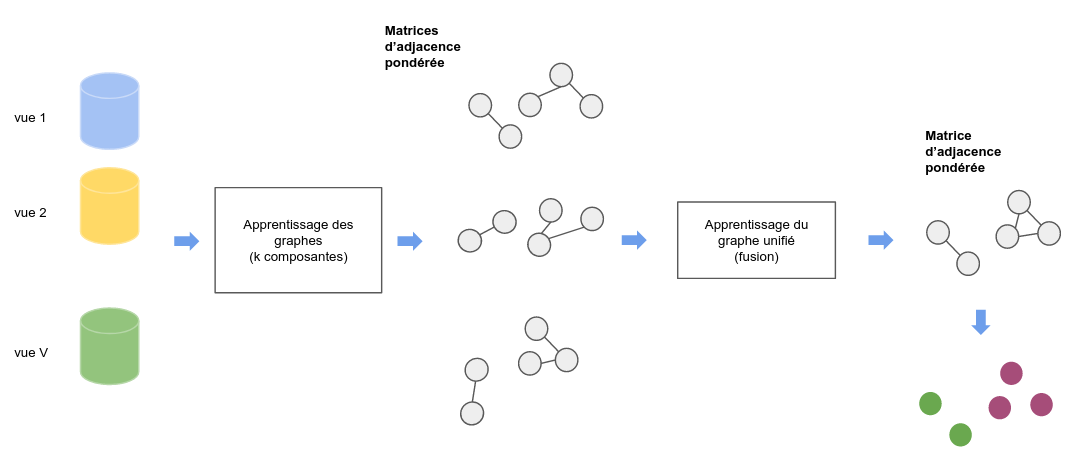
\includegraphics[width = \linewidth]{Images/mvgl1.png}
			\caption{Workflow de l'algorithme MVGL \cite{zhan2017graph}}
			\label{fig:mvgl2}
  	  \end{figure}

   	 Soit $K$ le nombre de clusters voulus.
   	 En supposant qu'un graphe dénué de biais de données est un graphe ayant déjà $K$ composantes connexes (clusters), on va en construire pour chacune des vues en s'appuyant sur leurs données.
  	 
   	 Pour chaque vue $v$, considérons qu'on a une projection des observations nommée $Q$ tel que les vecteurs d'observations du même groupe sont très similaires et peu pour ceux de groupes différents; et une matrice $S$ d'adjacence du graphe voulu. On peut à cet effet voir la différence entre les vecteurs $q_i$ et $q_j$ de deux observations $i$ et $j$ associée à leur similarité $S_{ij}$ (si elles sont connectés), comme une erreur.
   	 Ce qui permet d'affirmer qu'en minimisant la somme de ces différences pondérés pour tous les couples d'observations, on calcule simultanément ces vecteurs indicateurs et la matrice d'adjacence du graphe.
% On va ainsi s’assurer que le graphe ai $K$ composantes connexes, en calculant itérativement $S$ et $Q$ tant que la somme des $K$ plus petites valeurs propres du laplacien du graphe n'est pas égale à 0. Cela en s'appuyant sur le théorème suivant (Mohar et al. 1991):

   	 % \justify \textbf{Théorème 1} : La multiplicité $c$ de la valeur propre $0$ du laplacien d'un graphe est égale au nombre de composantes connexes de ce graphe.
  	 
           Plus formellement pour chaque vue $v$, on construit un graphe de matrice d'adjacence $S^{(v)}$ avec les vecteurs indicateurs $Q^v$, en résolvant le problème d'optimisation suivant où $S$ correspond à $S^{(v)}$, $Q$ à l'indicateur de clusters pour la vue, $L = D - \frac{(S + S^T)}{2}$ au laplacien du graphe avec $D$ étant la matrice de degré de $\frac{(S + S^T)}{2}$,
  	  et $j$ étant l'indice d'une observation.
    
           \begin{equation}
			\begin{aligned}
				& \min_{Q,S} \text{Tr}(Q^TLQ) + \beta{||S||}_F^2
     		   \\ & \text{s.t.}\ \forall j,\ \textbf{1}^Ts_{.j} = 1,\ s_j\geq0 , Q^TQ = I
     	   \end{aligned}
			\label{equa:mvgl1}
  	  \end{equation}
    
  	  D'où l'algorithme:
  	  \begin{algorithm}[H]
      		 \caption{Algorithme d'apprentissage des graphes des vues \cite{zhan2017graph}}
      		 \label{alg:mvgl1}
      		 \begin{algorithmic}[1]
      		 \REQUIRE Données d'entrée $X = \{ X^{(1)}, X^{(2)},\dots,X^{(V)} \}$, la constante de régularisation $\beta$, $k$ le nombre de clusters
     		 \STATE Initialiser pour chaque vue $v$, $Q^{(v)}$ avec $X^{(v)}$,
		      \FOR{$v \in [1,V]$}
     	 		 \REPEAT
					\STATE résoudre le problème \ref{equa:mvgl1} avec pour seul variable $S^{(v)}$
           		 \STATE résoudre le problème \ref{equa:mvgl1} avec pour seul variable $Q^{(v)}$
       		 \UNTIL{$S^{(v)}$ a $k$ composantes connexes}
			\ENDFOR
   		 \STATE retourner $S$, $Q$
   		 \end{algorithmic}
   	 \end{algorithm}

		 En développant le problème \ref{equa:mvgl1} en considération comme seul variable $S$, on obtient le problème quadratique suivant à résoudre:
   	 
		 \begin{equation}
			\begin{aligned}
				& \min_{s_j} {\left\| s_{j} + \frac{1}{2\beta}g_j \right\|}_2^2
     		   \\ & \text{s.t.}\ \forall j,\ \textbf{1}^Ts_{j} = 1,\ s_{j}\geq0
     	   \end{aligned}
  	  \end{equation}
		 où $g_{ij} = {|| q_i - q_j ||}^2$
   	 
		 Pour résoudre le problème \ref{equa:mvgl1} en considérant comme unique variable $Q$, on retrouve par développement de la relation de nullité du gradient lagrangien (des conditions de KKT) la variable optimal $Q^*$. $Q^*$ étant constitué les $K$ premiers vecteurs propres du laplacien du graphe issu de $S$, selon l'ordre croissant de leur valeur propre, avec $K$ étant le nombre de clusters voulus. %Cela en s'appuyant sur le théorème suivant (Mohar et al. 1991):

   	 %\justify \textbf{Théorème 1} : La multiplicité $c$ de la valeur propre $0$ du laplacien d'un graphe est égale au nombre de composantes connexes de ce graphe.
  	 
   	 Pour fusionner les graphes des vues, il suffit pour chaque couple d'observations, de sommer pourcentages des poids des arêtes les liant dans les graphes des vues.
   	 En considérant que la matrice d'adjacence $A$ du graphe globale peut être donnée, la différence entre elle et la somme pondérée des matrices d'adjacence des graphes des vues peut être vue comme une erreur.
  	 
   	 Dans le même principe de construction des graphes des vues, on considère une matrice indicatrice $P$ des observations de tel sorte que les vecteurs d'observations de même groupe sont très similaires et peu pour celles de groupe différent. On revoit ainsi la différence entre deux vecteurs $p_i$ et $p_j$ de deux observations $i$ et $j$ pondérée par leur similarité $a_{ij}$ (si elles sont connectées) comme une erreur.

  	  Plus formellement, pour construire le graphe unifié des graphes uniques à chaque vue, on résout le problème d'optimisation suivant, où
  	  $A$ correspond à la matrice d'adjacence du graphe globale,
        $P$ à l'indicateur de clusters globale et
  	  $W$ aux poids d'influence pour chacune des vues sur chacune des observations.
        \begin{equation}
			\begin{aligned}
				& \min_{A,W,P} \sum_{j=1}^n {\left\| a_{j} - \sum_{v=1}^V w_{j}^{(v)}s_{j}^{(v)}\right\|}_2^2 + \gamma \text{Tr}(P^TLP)
     		   \\ & \text{s.t.}\ \forall j,\ \textbf{1}^Ta_{j} = 1,\ a_{.j}\geq0,\ \sum_{v=1}^V w_{j}^{(v)} = 1
     		   \\ & P \in \mathbb{R}^{k \times n} ,\ P^TP = I
     	   \end{aligned}
			\label{equa:mvgl2}
  	  \end{equation}
      
        D'où l'algorithme:
  	  \begin{algorithm}[H]
     	   \caption{Algorithme d'apprentissage du graphe globale \cite{zhan2017graph} }
     	   \label{alg:mcles1}
     	   \begin{algorithmic}[1]
     	   \REQUIRE Les matrices de similarité des graphes des vues $S = \{ S^{(1)}, S^{(2)},\dots,S^{(V)} \}$, la constante de régularisation $\gamma$, $k$ le nombre de clusters
     	   \STATE Initialiser $W = \frac{1}{V}$, $a_j = \sum_{v=1}^V w_j^{(v)}s_j^{(v)}$
 		 \STATE résoudre le problème \ref{equa:mvgl2} avec pour seul variable $P$
     	   \WHILE{il n'y a pas de convergence}
     		   \REPEAT
 				   \STATE résoudre le problème \ref{equa:mvgl2} avec pour seul variable $A$
 				   \STATE résoudre le problème \ref{equa:mvgl2} avec pour seul variable $P$
     		   \UNTIL{ A a $k$ composantes connexes }
		   	   \STATE résoudre le problème \ref{equa:mvgl2} avec pour seul variables $W$
     	   \ENDWHILE
     	   \STATE retourner $A$,$P$,$W$
     	   \end{algorithmic}
        \end{algorithm}

   	 En développant le problème \ref{equa:mvgl2} en considérant comme unique variable $A$, on obtient le problème quadratique suivant:
   	 \begin{equation}
			\begin{aligned}
				& \min_{a_j} {\left\| a_{j} + \left( \frac{1}{2\beta}h_{j} - \sum_{v=1}^V w_{j}^{(v)}s_{j}^{(v)}  \right) \right\|}_2^2
     		   \\ & \text{s.t.}\ \forall j,\ \textbf{1}^Ta_{j} = 1,\ a_{j}\geq0
     	   \end{aligned}
  	  \end{equation}
		 où $h_{ij} = {|| p_i - p_j ||}^2$
   	 
		 La résolution du problème \ref{equa:mvgl2} en considérant comme unique variable $P$, est la même que pour celui du problème \ref{equa:mvgl1} avec pour unique variable $Q$, en voyant $Q$ comme $P$ et $S$ comme $A$.

		 Pour résoudre ce même problème en considérant $W$ comme unique variable, on développe la condition de nullité du gradient lagrangien (des conditions de KKT) afin d'obtenir la relation suivante :
		 \begin{equation}
			  w_j = \frac{ {\left( Z_{j}^{T}Z_{j} \right)}^{-1} 1 }{ 1^T {\left( Z_{j}^{T}Z_{j} \right)}^{-1} 1}
  	  \end{equation}
   	 où $z_{j}^{(v)} = a_j - s_{j}^{(v)}$
    
      
	\section{Algorithmes d'ensemble de clustering}
    
  	  Construire des clusters issues de ceux de base (issus des algorithmes de base), revient à construire un ensemble $C$ de $K$ clusters qui se rapprocheront le mieux possible de ceux de base.
  	  En d'autres termes on souhaite un ensemble de clusters final, qui aura un minimum de désagrément avec les clusters de base.
  	  De là, on peut se rendre compte que la principale difficulté à franchir est celle de trouver les correspondances entre les différents clusters de base.
  	  Dans le but de le faire, plusieurs approches ont été proposées dont les suivantes.
    
       \subsection{Algorithmes de correspondance forte}
      
  	  L'idée de ces algorithmes est de rechercher la correspondance entre les clusters de weak-learners différents
  	  en supposant qu'on a pour chaque cluster d'un weak-learner son correspondant dans un autre weak-learner.
  	  On peut donc voir que cela conduit à trouver un ré-ordonnancement, une permutation entre les clusters de différents weak-learners, qui permet d'avoir le consensus le plus élevé entre les clusters des weak-learners. La figure \ref{fig:ens2} illustre le principe.
    
  	  \begin{figure}
     	   \centering
     	   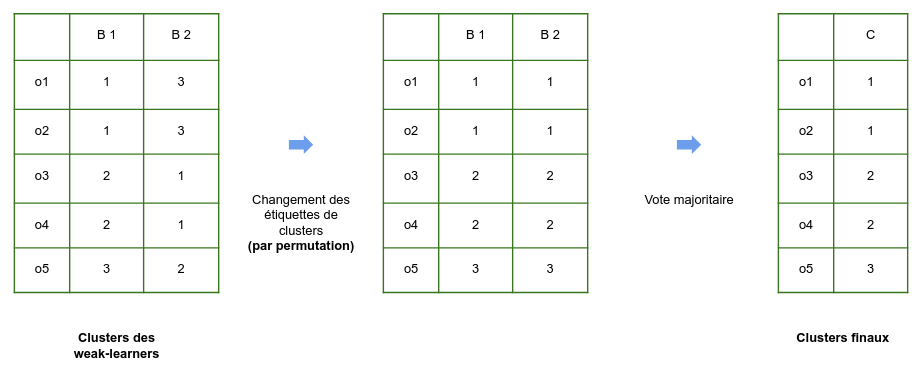
\includegraphics[width = 0.7\linewidth]{Images/ens2.png}
     	   \caption{Processus général des algorithmes de correspondance forte}
     	   \label{fig:ens2}
        \end{figure}
  	  On peut citer les travaux de Sandrine Dudoit et Jane Fridlyand \cite{dudoit2003bagging} qui ont proposés deux versions de l'algorithme Bagging dans ce sens.
   
  	  \subsection{Algorithmes de correspondance légère}
      
  	  Pour réduire le temps du calcul des algorithmes de correspondance forte,
  	  On pourrait calculer des correspondances plus légères entre les clusters de chaque weak-learner. Pour le faire, ces algorithmes passent généralement par la formulation qui suit:
           soient $S(m)$ la matrice de correspondance entre les clusters du $m-ème$ weak-learner et les clusters finaux, de tel sorte que
  	  $S_{k',k}(m) = 1$ si le cluster $k'$ du weak-learner $m$ de base correspond au cluster finale $k$,
  	  $S_{k',k}(m) = 0$ sinon; $M(m)$ comme étant la matrice d'assignation des observations aux clusters du $m-ème$ weak-learner où
  	  $M_{i,k'}(m) = 1$ si l'observation $i$ est dans le cluster $k'$ du weak-learner de base,
  	  $M_{i,k'}(m) = 0$ sinon; et $C$ la matrice d'assignation des observations aux clusters finaux.
  	  On a ainsi le problème d'optimisation générale suivant :
  	  \begin{equation}
  		  \min {\| C - MS \|}^2
  	  \end{equation}

  	  Pour résoudre ce problème, on utilise généralement l'algorithme EM %\cite{long2005combining}
      où les matrices de correspondance sont les variables cachées et la matrice d'assignation est la variable qu'on recherche.
    
  	  \subsection{Algorithmes basés sur les observations}
      
  	  L'idée ici est de représenter une observation, par l'ensemble des étiquettes de clusters dans lesquels il se trouve. Ce qui permet de construire de nouveaux clusters grâce à l'utilisation d'un second algorithme de clustering.
    
  	  % De là on peut définir, la similarité entre deux observations comme étant le pourcentage de weak-learners qui les assignent dans le même cluster; et la dissimilarité entre eux comme étant le pourcentage de weak-learners qui ne les assignent pas dans le même cluster.
    
  	  Ce second algorithme de clustering ayant principalement pour but de construire les clusters finaux de consensus, on définit généralement des fonctions pour l'évaluer:
  	  \begin{itemize}
  		  \item La moyenne des informations mutuelles normalisées entre les clusters finaux et les clusters de base décrit dans \cite{strehl2002cluster}, avec $M$ le nombre de weak-learners, $C$ la colonne d'étiquettes de clusters globaux, $B(m)$ la colonne d'étiquettes de clusters du weak-learner $m$
  		  \begin{equation}
  			  \max_C \frac{1}{M}\sum_{m=1}^{M} NMI(C, B(m))
  		  \end{equation}
  		  \item La fonction objective du clustering de corrélation décrit dans \cite{gionis2007clustering}, avec $S_{ij}$ étant le nombre de clusters de base où on retrouve les observations $i$ et $j$ simultanément
  		  \begin{equation}
  			  \max \sum_{i,j \text{, } C(i)=C(j)} (1 - S_{i,j}) + \sum_{{i,j} \text{, } C(i) \neq C(j)}  S_{i,j}
  		  \end{equation}
  	  \end{itemize}
 	 
  	  Comme second algorithme de clustering, on a généralement:
  	  \begin{itemize}
  		  \item Algorithme de clustering hiérarchique \cite{gionis2007clustering}: \acrshort{CAH}, \acrshort{CDH}

  		  \item Algorithme LocalSearch modifié \cite{gionis2007clustering}:
  		  on initialise au départ éventuellement les clusters aléatoirement, puis on change le cluster d'une observation,
  		  si en le faisant la valeur de la fonction objective s'améliore, on le fera tant qu'il est possible d'améliorer la fonction objective
    
  		  \item Algorithmes de partitionnement de graphes: \acrfull{CSPA}, \dots
  		  Ici on réalise le partitionnement du graphe des données où un nœud est une observation et une arête porte la similarité entre observations.
     	 
  		  \item L'algorithme \arcshort{EM} modifié %\cite{topchy2005clustering}
          pour des distributions multinomiaux
  	  \end{itemize}

      
  	  \subsection{Algorithmes basés sur les clusters}
      
  	  Dans l'optique de s'appuyer directement sur les clusters de base, on représente chacun d'eux comme un vecteur binaire d'appartenance des observations.
  	  Puis on les regroupe en un nombre donnée de groupes finaux de clusters,
  	  puis on assigne chaque observation au groupe de clusters qui possède le plus de clusters le contenant.
  	  On peut citer les algorithmes \acrfull{MCLA}\cite{strehl2002cluster} et \acrfull{ACE}\cite{alqurashi2019clustering}.
      
  	  \subsection{Algorithmes basés sur les clusters et les observations}
      
  	  L'idée est de tenir compte des observations et des clusters pour construire les clusters finaux en les représentant dans une structure commune.
  	  Généralement on les représentent en deux types de graphe:
  	  \begin{itemize}
  		  \item hyper-graphe :
  		  ici un noeud est une observation et une hyper-arête est un cluster de base
  		  \item graphe bipartie :
  		  ici on a deux ensembles de noeuds, l'ensemble des noeuds des observations et l'ensemble des noeuds des clusters de base,
  		  une arête est la liaison entre une observation et un cluster de base qui le contient.
  	  \end{itemize}
  	  Ces graphes permettent par leur coupure d'obtenir les $K$ clusters finaux recherchés.
    
  	  Par exemple, l'algorithme HGPA \cite{strehl2002cluster} représente les clusters de base et les observations avec un hypergraphe.

      
  	  \subsection{Comparaison des algorithmes d'ensemble de clustering}

  	  Nous avons le tableau \ref{tab:comp_ens} de comparaison suivant mettant en évidence les avantages et limites des algorithmes en se basant sur leurs propriétés

  	  {\begin{longtable}{|p{4.5cm}|p{6cm}|p{6cm}|}
  		  \caption{Tableau de comparaison des algorithmes d'ensemble de clustering}
  		  \label{tab:comp_ens}
  			  \hline
 				   \textbf{Algorithme} & \textbf{Avantages} & \textbf{Limites} \\
  			  \hline
     				   Algorithmes de correspondance forte
     				   &
     				   {- ils permettent d'avoir les correspondances entre les regroupements de base}
     				   &
          			  {- ils nécessitent que chaque weak-learner retourne un même nombre de clusters} \newline\newline
     				   {- ils sont coûteuses en temps à cause la recherche des correspondances par permutation}
     				   \\
  			  \hline
     				   Algorithmes de correspondance légère
     				   &
     				   {- ils prennent en considération le fait que chaque weak-learner peuvent fournir des nombres différents de cluster}
     				   &
     				   {- Deux clusters d'un même weak-learner de base peuvent correspondrent à un même cluster finale} \newline\newline
          			  {- La ressemblance entre les clusters de weak-learners différents ne sont pas réellement pris en compte}
          			  {}
     				   \\
  			  \hline
     				   Algorithmes basés sur les observations
     				   &
     				   {- Ces méthodes tiennent compte du fait que les weak-learners de base peuvent fournir des clusters de nombres différents} \newline\newline
     				   &
          			  {- d'après les opérations qu'ils utilisent, ils prennent beaucoup de temps lorsqu'on a beaucoup d'observations} \newline\newline
          			  {- ils sont sensibles à une grande variabilité de la constitution des clusters des différents weak-learners} \newline\newline
          			  {- ils dépendent généralement de métriques de dissimilarité et de similarité utilisées}
     				   \\
  			  \hline
     				   Algorithmes basés sur les clusters
     				   &
     				   {- ils tiennent compte du fait qu'une observation ne soit pas assigner à un cluster par au moins un weak-learner} \newline\newline
     				   {- ils assignent les observations à des groupes de clusters grâce à leur occurrence et dont s'attèlent au vote majoritaire} \newline\newline
          			  {- ils sont moins sensibles à une grande variabilité de la constitution des clusters des différents weak-learners} \newline\newline
          			  {- ils tiennent compte de la ressemblance des clusters de base}

     				   &
     				   {- ils dépendent généralement de métriques de dissimilarité et de similarité utilisées}
     				   \\
  			  \hline
     				   Algorithmes basés sur les clusters et les observations
     				   &
     				   {- ils intègrent les clusters de base et les observations simultanément } \newline\newline
          			  {- ils permettent de réduire la dimensionnalité des données d'origine }
     				   &
     				   {- Ils sont sensibles à une grande variabilité de la constitution des clusters des différents weak-learners}
     				   \\
  			  \hline
  		  \end{longtable}
  		  }

  	  De ces comparaisons, nous voyons que les algorithmes basés sur les clusters se rapprochent plus du vote majoritaire des méthodes d'apprentissage ensemblistes.
  	  Nous présenterons ainsi par la suite les algorithmes \acrshort{ACE} et \acrshort{MCLA} qui font partie des plus performant de cette catégorie.
      
  	  \subsection{\acrfull{ACE}}

  		  L'idée ici est de construire les clusters finaux par fusion des clusters de base similaire et d'attribuer les observations à ces clusters grâce à leurs pourcentages d'appartenance, en utilisant des seuils de similarité adaptés au besoin.
     	   Pour le faire l'algorithme ACE, suit trois étapes qui sont visibles sur la Figure \ref{fig:ace1}:
     	 
     	   % figure ace_workflow.png
     	   \begin{figure}
     		   \centering
     		   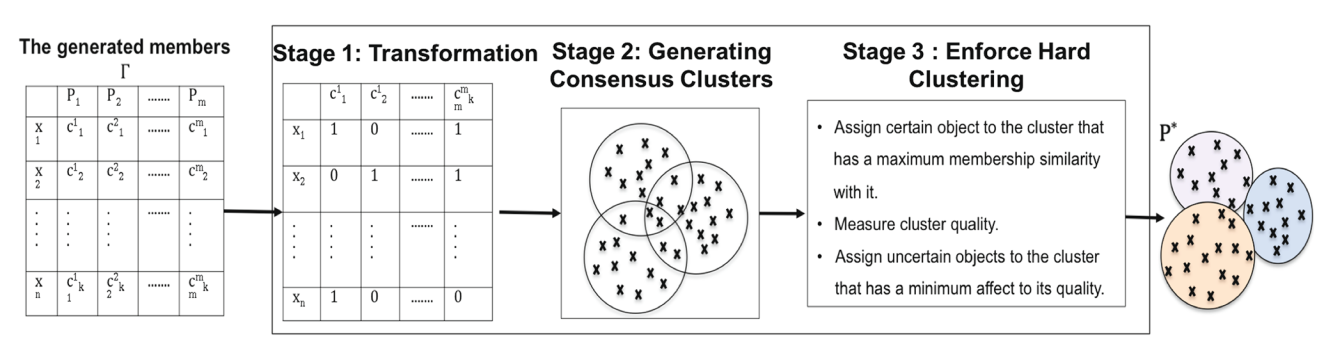
\includegraphics[width = \linewidth]{Images/ace_workflow.png}
     		   \caption{Processus de l'algorithme ACE \cite{alqurashi2019clustering}}
     		   \label{fig:ace1}
     	   \end{figure}
      
     	   \begin{enumerate}
     		   \item \textbf{Transformation des clusters issues des algorithmes de base}
			 
     		   Cette étape consiste à transformer chaque cluster de base en un vecteur binaire où la $i$-eme composante est égale à $1$ si l'observation $i$ est dans le cluster, et $0$ sinon
			 
     		   \item \textbf{Calcul des $K$ groupes de clusters de consensus}
			 
     		   Cette étape consiste à construire $K$ groupes des clusters de base (méta-cluster) en deux temps.
			 
     		   Dans un premier temps, on regroupe les couples de clusters qui ont une similarité (coefficient de Pearson %\cite{houle2008relevant})
               supérieur à un seuil donné $\alpha_1$ adapté pour obtenir au moins $K$ groupes.
  	 
     		  Dans un second temps, on va vérifier si $K$ méta-clusters ont chacun au moins une observation certaine de leur appartenir.
    		 Une observation est certaine d'appartenir à un méta-cluster si sa similarité d'appartenance au méta-cluster (mesurée en utilisant la formule \ref{equa:ace2}) dépasse un seuil $\alpha_2$ donné.
     		   Si c'est le cas, on considère ces méta-clusters comme groupes à exploiter, sinon on considérera plutôt les $K$ méta-clusters qui ont les plus grandes moyennes de similarité d'appartenance d'observations.
			 
     		   \item \textbf{Assignation des observations aux groupes (méta-clusters)}
			 
     		   Cette étape consiste à construire les clusters finaux, en assignant les observations aux $K$ groupes obtenus qui peuvent être vus comme des clusters.
     		   Cela s'effectue, en assignant les observations aux groupes auxquelles elles sont certaines d'appartenir.
     		   Les autres observations seront ajoutées aux clusters dont elles perturberont le moins la qualité.
     		   La qualité de groupe étant calculée en évaluant la variance des similarités d'appartenance des observations d'un groupe, de formule \ref{equa:ace3}.
			 
     	   \end{enumerate}
      
     	   Il faut noter que la similarité d'appartenance d'une observation $i$ à un groupe $g$ correspond au pourcentage du nombre de clusters du groupe, dans lesquels elle a été retrouvée.
     	   \begin{equation}
     		   S_x(x_i,c_g) = \frac{\theta(x_i, c_g)}{ max\{ \theta(x_i, C) \} }
     		   \label{equa:ace2}
     	   \end{equation}
     	   avec, $x_i$ étant la $i$-ème observation, $c_g$ étant le $g$-ème groupe de clusters, $C$ étant l'ensemble des groupes de clusters, $\theta(x_i, c_g)$ étant le nombre de clusters de $c_g$ où on trouve l'observation.
      
     	   De plus la qualité d'un groupe $c$ est la variance $\text{Var}(c)$ des similarités d'appartenance de ces observations, on a:
     	   \begin{equation}
     		   \text{Var}(c) = \frac{1}{ \|c\|} \sum_{i=1}^{\|c\|} (S_x(x_i,c) - \rho_c)
     		   \label{equa:ace3}
     	   \end{equation}
     	   avec $\rho_c$ la moyenne de similarité d'appartenance d'observations du groupe $c$.
  	 
      
     	   \subsection{\acrfull{MCLA}}

  	 
     	   L'idée de l'algorithme est de regrouper les clusters de base en $K$ groupes de clusters appelés méta-clusters, puis d'assigner chaque observation au méta-cluster qui possède le plus de clusters le contenant.
     	   Pour le faire l'algorithme MCLA suit les étapes suivantes:
     	 
     	   \begin{enumerate}
     		   \item \textbf{Transformation des clusters de base}
  		 
     		   Cette étape consiste à transformer chaque cluster de base en un vecteur binaire où la i-eme composante est égale à 1 si l’observation i est dans le cluster, et 0 sinon
      
     		   \item \textbf{Construction du graphe de similarité de ces clusters}
     	 
     		   Cette étape consiste à construire un graphe, où les sommets sont les clusters de base, et où les arêtes portent les similarités entre ces clusters.
     		   La similarité entre deux clusters étant mesurée par l'indice de Jaccard de ces derniers, qui est décrit comme suit:
			 
     		   Soit $a$ et $b$ étant des clusters de base, l'indice de Jaccard $S(a, b)$ entre eux, est calculé en utilisant la formule suivante:
     		   \begin{equation}
					S(a, b) = \frac{|a \cap b|}{|a \cup b|} = \frac{h_a^{\small{T}} h_b}{\|h_a\|_2^2 + \|h_b\|_2^2 - h_a^{\small{T}} h_b}
				\end{equation}
     		   avec $h_a$ et $h_b$ étant les vecteurs binaires des clusters $a$ et $b$ respectivement
      
     		   \item \textbf{Regroupement des clusters en $K$ méta-clusters}
			 
     		   Cette étape consiste à regrouper les clusters en $K$ groupes de clusters similaires appelés méta-clusters.
     		   Pour le faire, on réalise une coupure du graphe de similarité obtenu à l'étape précédente, en utilisant METIS %\cite{karypis1995multilevel}.
  	 
            	METIS procède en trois étapes principaux: il réduit la taille du graphe en fusionnant successivement des noeuds adjacents en des multi-noeuds, il partitionne le graphe obtenu avec des algorithmes tel que l'algorithme de partitionnement spectral, et étend au final ce partitionnement au graphe d'origine par segmentation des multi-noeuds construits et affection des noeuds aux clusters formés.
		 
     		   On pourra ainsi en pratique pour chaque groupe obtenu, sommer les vecteurs binaires de ses clusters, pour compter pour chaque observation, le nombre de clusters du groupe qui lui contiennent.
      
     		   \item \textbf{Construction des clusters finaux}
			 
     		   Cette étape consiste à attribuer chaque observation au méta-cluster qui possède le plus de clusters de base le contenant.
      
     	   \end{enumerate}

  	  Des deux algorithmes précédents, MCLA par son processus se rapproche le plus du vote majoritaire des algorithmes d'apprentissage par ensemble, qui permet de rendre plus robuste le modèle globale et de réduire le risque de sur-apprentissage.
    
   	 En somme, il était question pour nous de faire un état des algorithmes à notre connaissance qui permettent d'avoir des briques de réponse à la question de recherche posée. Nous pouvons citer les algorithmes de clustering à une vue, de clustering multi-vues et d'ensemble de clustering. Au vue des caractéristiques propres aux données spectrales (comme la présence de biais) et de la nature des réseaux moléculaires, nous avons présenté plus en détail les algorithmes de clustering \acrshort{DBSCAN}, \acrshort{SCAN}, \acrshort{NSDBSCAN}; de clustering multi-vues \acrshort{MCLES} et \acrshort{MVGL}; et d'ensemble de clustering \acrshort{ACE} et \acrshort{MCLA}.
   	 Dans les lignes qui suivent nous proposerons des algorithmes basés sur les algorithmes d'apprentissage par ensemble Bagging et Boosting pour atteindre l’objectif fixé.
  	 
    \input{Chapitre3-4}
    \chapter{Conclusion Générale}


Dans cette étude, nous avons considéré la complémentarité et le potentiel consensus d'informations qui existent entre les spectres MS et RMN des molécules. Cela dans le but d'identifier les molécules qui ne le sont pas et donc d'identifier les réseaux moléculaires les contenant.
Les méthodes existantes telles que GNPS et MADByTE utilisant respectivement les spectres MS et RMN, ne prennent pas en compte cette complémentarité et ce consensus d'informations obtenus des molécules par spectrométrie.
Pour pouvoir les exploiter pour la construction des réseaux issus respectivement de GNPS et de MADByTE, nous avons combiner les clusters dans ces réseaux avec ceux obtenus par le biais des algorithmes de clustering multi-vues MCLES ou MVGL, par apprentissages par ensemble Bagging et Boosting, avec comme algorithme de vote majoritaire MCLA.
Pour obtenir automatiquement les clusters contenus dans les réseaux, nous avons utilisé l'algorithme DBSCAN en définissant le voisinage d'une molécule dans un réseau moléculaire.

Nos expérimentations sur la dataset MSRC-V1, ont permis d'observer qu'avec MCLES comme weak-learner, nous avons les meilleures performances en termes de regroupement. On parle de 80.1\% d'exactitude, 74.3\% d'information mutuelle normalisée et de 81.1\% de pureté pour le Bagging. Cela montre que les clusters construits par apprentissage ensembliste tiennent mieux compte des structures complexes des données. Ce qui nous permet d’affirmer que l’approche basée sur les apprentissages Bagging et Boosting améliorent la qualité des réseaux moléculaires qui accéléra leurs processus d'identification.

Néanmoins, nous avons été confrontés à des difficultés qui nous ont permis de cerner des limites à l'approche. Premièrement toutes les approches proposées ont besoin de données complètes des spectres MS et RMN qui se trouvent très difficile à avoir en pratique, ensuite le temps d'exécution est relativement grand et enfin les approches proposées accordent la même importance aux données de chaque représentation malgré le fait que les spectres MS contiennent beaucoup plus de bruits que les spectres RMN.
De là, nous comptons pour la suite, en premier lieu expérimenter les approches proposées complètement sur des spectres de molécules issus de notre propre collecte des données, puis d'accélérer les approches par parallélisation, et d'enfin proposer une méthode prenant en compte l'importance que doit avoir les spectres MS et RMN chacune dans la construction d'une représentation unifiée pour améliorer le clustering.

\justify



    
    \newpage
    %\pagenumbering{roman}
    \addcontentsline{toc}{chapter}{Bibliographie}
      \bibliographystyle{unsrt}
    \bibliography{reference_GNPS_MADByTE}

%\newpage
%\addcontentsline{toc}{chapter}{Autres références}
%\bibliographystyleother{plain}
%\bibliographyother{references/Bibliographie}


%\newpage
%\pagenumbering{roman}
%\input{Annexe/Annexe}


\end{document}
